\documentclass[twoside]{article}
\input{ISC18-english.sty}
%%%%%%%%%%%%%%%%%%%%%%%%%%%%  Make sure to compile twice for proper cross-references. %%%%%%%%%%%%%%%%%%%%%%%
%%%%%%% For proper display of references, compile the document twice. %%%%%%%%%%%%%%%%%%%%% 
%%%%%%%%%%%%%%% If using TeX Live, compile using pdflatex command %%%%%%%%%%%%%%%%%%%%%%%



\begin{document}
	\thispagestyle{empty}
	%%%%%%%%%%%%%%%%% Article title header  %%%%%%%%%%%%%%%%%%%%
	\fancyhead[LE]{Graph Feature Extraction for Path Planning Using Machine Learning SVM and GNN}
	%%%%%%%%%%%%%%%%% Article authors header   %%%%%%%%%%%%%%%%%%%%
	\fancyhead[RO]{Abdolhosseinzadeh, Emami, Azarnavid}
	\begin{center}
		{
\includegraphics [height=25mm, width=150.3mm] {Images/isc18E}} \\
		\vspace*{-1.8cm}
		\vspace*{4cm}
		%%%%%%%%%%%%%%%%% Article title  %%%%%%%%%%%%%%%%%%%%
		{\Large \bf Graph Feature Extraction for Path Planning Using Machine Learning by SVM and GNN}\\
		%%%%%%%%%%%%%%%%% Article authors and affiliations %%%%%%%%%%%%%%%%%%%%
		{\bf
			Mohsen Abdolhosseinzadeh\footnote[1]{{\bf Corresponding Author:} {\tt mohsenab.ubonab@gmail.com }} , Hojjat Emami$^2$, Babak Azarnavid$^3$  \\
			$^{1,3}$Department of Mathematics and Computer Science, University of Bonab, Bonab, Iran \\
			$^2$Department of Computer Engineering, University of Bonab, Bonab, Iran}
	\end{center}
	\rule{\textwidth}{0.2mm}\\
	%%%%%%%%%%%%%%%%% Article abstract  %%%%%%%%%%%%%%%%%%%%
	\noindent{\bf Abstract:}\\
	 This paper surveys how machine learning, particularly graph neural networks and transformer architectures, automates the extraction of features to improve path planning processes. We characterize the methodological development from traditional topological invariant graph features to advanced data-driven representation learning frameworks, demonstrating their efficacy in optimizing navigation policies across complex, stochastic, and multi-agent operational domains. Furthermore, the practical realities of implementing these models are addressed, focusing on computational limits at the edge, real-world execution, and enhancing models in operational settings. Finally, experimental results are provided supporting the efficacy of the proposed graph feature extraction framework in reducing node expansions and improving path optimality across a variety of path planning benchmarks.

	

	\noindent{\bf Keywords:} 
	Path planning, Graph Neural Networks, Heuristic learning, Problem reduction. \\
	\noindent{\bf Mathematics Subject Classification (2010):} $\rm 68T20$, $\rm 68T05$, $\rm 90C27$. \\
	\hspace{1cm}\rule{\textwidth}{0.2mm}\\
	%%%%%%%%%%%%%%
	\section{Introduction}

	

	Machine learning provides a systematic alternative to hand-crafted feature engineering by learning latent representations directly from observational data. When the environment is modeled as a graph, Graph Neural Networks and their architectural successors can extract topological, geometric, and semantic features that are strongly predictive of path planning performance, as demonstrated in foundational value iteration networks \cite{tamar2016} and subsequent neural search paradigms \cite{yonetani2021, li2018combinatorial}. This research offers a comprehensive treatment of neural path planning, examining its mathematical foundations, modern architectures, multi-agent extensions, and practical deployment considerations. The primary contribution lies in presenting a unified framework that bridges classical statistical problem reduction with modern topology-aware deep learning. %We rigorously formalize discrete graph search, continuous configuration spaces, and partially observable decision processes under a single coherent feature extraction model. Building on this foundation, we analyze advanced architectures that mitigate over-squashing and over-smoothing in message-passing networks while detailing the mechanics of Graph Transformers. Beyond theoretical advances, we address critical deployment realities often overlooked in the literature, including edge-compute latency constraints, ROS2 middleware integration, and sim-to-real transfer via domain randomization. Finally, we explore emerging frontiers at the intersection of Graph-Retrieval-Augmented Generation, Large Language Models, and neuro-symbolic planning as promising directions for interpretable and adaptive autonomous navigation.

	

	%----------------------------------------------------
	\section{Path Planning and Problem Formulation}
	We model the path planning environment not merely as a static topology, but as a rich, attributed decision space. Formally, let the operational domain be represented by the weighted graph $G = (V, E, \mathbf{X}, \mathbf{E}_{feat}, \mathbf{A})$. The node set $V = \{v_1, \dots, v_N\}$ encodes discrete states or spatial regions, while the edge set $E \subseteq V \times V$ captures feasible transitions between them. This representation extends beyond simple connectivity through the matrix $\mathbf{X} \in \mathbb{R}^{N \times F_v}$, which embeds semantic and geometric context at each state, and $\mathbf{E}_{feat} \in \mathbb{R}^{|E| \times F_e}$, which characterizes transition-specific attributes such as surface friction, slope gradient, or regulatory restrictions. The adjacency matrix $\mathbf{A} \in \mathbb{R}^{N \times N}$ quantifies the nominal cost or capacity of each arc, serving as the baseline for optimization. 	
	Within this framework, a feasible path $\pi = (v_0, v_1, \dots, v_{|\pi|})$ is defined as an ordered sequence connecting the origin $v_0 = v_{start}$ to the destination $v_{|\pi|} = v_{goal}$, where $|\pi|$ is the number of edges in the path $\pi$. The path planning problem is then cast as a constrained combinatorial optimization task seeking the optimal policy $\pi^*$ that minimizes a composite objective:
	\begin{equation}\label{eq:path_cost}
		\pi^* = \arg\min_{\pi \in \Pi} \left[ \sum_{k=0}^{|\pi|-1} c(v_k, v_{k+1}, \mathbf{x}_{v_k}, \mathbf{e}_{v_k, v_{k+1}}) + \lambda \mathcal{R}(\pi) \right].
	\end{equation}
	This formulation deliberately decouples local and global performance criteria. The term $c(\cdot)$ represents the stage-wise transition cost, explicitly conditioned on both nodal state features and edge attributes, thereby allowing the cost structure to adapt dynamically to environmental semantics rather than relying on static geometric proxies. Simultaneously, the regularizer $\mathcal{R}(\pi)$ enforces system-level operational constraints and preferences, penalizing excessive curvature, proximity to hazards, energy inefficiency, or violation of safety corridors. The scalar weight $\lambda \geq 0$ governs the trade-off between nominal traversal cost and these higher-order behavioral requirements, effectively embedding multi-criteria decision-making into a single scalarized objective amenable to standard search or learning-based solvers. This unified cost structure is essential for ensuring that computed paths are not only geometrically valid but also operationally viable in complex, real-world deployment scenarios.

	

	%--------------------------------------------------
	\section{Statistical Feature Extraction for Graph Reduction}
	To complement deep representation learning, we incorporate a statistical feature extraction framework inspired by Machine Learning for Problem Reduction (MLPR) \cite{Sun:2021, Stodola:2025}. This approach characterizes each edge $e_{i,j} \in E$ using computationally inexpensive descriptors that capture both local graph topology and global solution likelihood. Unlike learned embedding, these features are solver-agnostic, require no training, and enable aggressive pruning of irrelevant transitions prior to neural processing or search.

	

	We define four normalized local features based on the edge cost structure relative to local neighborhood statistics. These features capture the relative attractiveness of an edge within its immediate topological context and remain consistent with the transition cost defined in Equation~\eqref{eq:path_cost}. The first two features measure the normalized deviation of an edge cost from the minimum outgoing and incoming edge costs connected to its endpoints, while the third and fourth features measure deviation from the mean edge costs of the respective neighborhoods. All local features are normalized to the unit interval to prevent scale dominance during downstream learning or thresholding. %For sparse graphs, these local statistics are computed in linear time with respect to the edge count, making them suitable for real-time preprocessing.

	

	Beyond local geometry, we quantify the global relevance of each edge through stochastic sampling of feasible paths, as the next two global statistical features. Let $\{P_1, \dots, P_m\}$ denote $m$ randomly generated feasible routes. The first statistical measure is a ranking-based score that assigns higher values to edges frequently appearing in high-quality samples. We normalize this raw score by the maximum ranking-based score in the graph to maintain numerical stability. The second measure computes the Pearson correlation between edge presence and solution cost across samples. Since path planning is a minimization problem, edges that are negatively correlated with tour costs are more likely to belong to optimal solutions. Following the efficient set-based accumulation strategy proposed in the original MLPR framework \cite{Sun:2021}, both statistical measures are computed in $O(mn + |E|)$ time and space, avoiding the naive quadratic complexity.
	%with corresponding costs $\{y_1, \dots, y_m\}$.
	For uniformly random tours, the strong law of large numbers guarantees convergence of the rank-based score, with the Berry-Esseen theorem giving a rate of $O(m^{-1/2})$ as $m\rightarrow \infty$ \cite{Berry1941, Korolev2010}. %The correlation measure  is a consistent estimator of the population point-biserial correlation, and it effectively ranks edges by linear dependence with tour cost.

	

	These six features serve dual purposes in our framework, bridging classical problem reduction and modern neural path planning. The statistical descriptors first provide explicit optimality signals that ground latent representations, improving convergence and generalization to unseen topologies. They subsequently function as a pre-filtering mechanism that reduces the computational graph size before expensive neural inference or search. The total feature extraction cost remains negligible compared to GNN inference. In practice, the sample size is scaled linearly with graph dimension to ensure adequate edge coverage while maintaining sub-second preprocessing. %For dynamic environments, local features can be updated incrementally upon edge cost changes, while global sampling features are recomputed only when the cost landscape shifts significantly. This hybrid update strategy enables real-time adaptation without full resampling. It is worth noting that while MLPR features generalize well across problem sizes and characteristics \cite{Sun:2021}, their predictive accuracy degrades when test instances differ substantially from the sampling distribution. In highly heterogeneous environments, we recommend using these features as soft attention biases rather than hard pruning masks, preserving feasibility while still accelerating search.

		

	%---------------------------------------------------
	\section{Comparative Experimental Analysis}
	To validate the integrated pipeline, we conduct a systematic comparison between the solver-agnostic statistical MLPR framework, implemented via cost-sensitive Support Vector Machine classification, and the topology-aware Edge Classification Graph Neural Network, implemented via PyTorch Geometric. Experiments are performed on three TSPLIB benchmarks of increasing scale and structural complexity: gr17 ($n=17$, 136 edges) with explicit costs, and eil51 ($n=51$, 1,275 edges) and berlin52 ($n=52$, 1,326 edges) with Euclidean distance matrices. All experiments use $m=100n$ random samples with a fixed seed for statistical feature generation, and optimal tours verified against TSPLIB known optima \cite{reinelt1991tsplib}. The SVM baseline employs an RBF kernel with a false-negative penalty scaled inversely to the positive class ratio to compensate for extreme imbalance. The GNN architecture follows a three-layer Graph Attention network with four attention heads, hidden dimension sixty-four, batch normalization, and an edge-level multi-layer perceptron classifier. Training utilizes weighted binary cross-entropy loss with a position weight scaled to the class imbalance ratio, optimized via Adam over two hundred epochs. Results are averaged over five stratified train/test splits.

	

	 The GNN consistently outperforms the SVM baseline by two to four percentage points in recall and three to six points in precision. This performance gap reveals fundamental differences in how each model exploits available information. The SVM treats each edge as an independent instance characterized solely by its six-dimensional feature vector and cannot recognize that adjacent edges forming a coherent tour segment are jointly informative. In contrast, the GNN message-passing mechanism propagates optimality signals across hops, enabling it to learn structural dependencies such as degree-two constraints in optimal tours. While the SVM relies on the RBF kernel to capture nonlinear feature interactions implicitly, the GNN learns task-specific feature combinations through its edge-classifier layers. The performance gap widens slightly from gr17 to berlin52, suggesting that as graph size increases, the fraction of information captured by local features alone decreases, and the GNN ability to integrate global topological context through attention becomes increasingly valuable.	

	

	The ranking-based score consistently emerges as the single most discriminative feature across all instances. Optimal edges achieve substantially higher mean ranking scores compared to non-optimal edges, with separation factors increasing from 2.5 times for gr17 to 4.0 times for berlin52. The larger sample budget for eil51 and berlin52 provides tighter concentration of ranking scores around high-quality backbone edges. Local features show consistent but weaker discrimination, confirming that global sampling statistics carry the primary optimality signal. The confusion matrices and ROC curves presented in Figures~\ref{fig:gnn_evaluation} and \ref{fig:svm_evaluation} further illustrate these findings. The GNN confusion matrices demonstrate near-perfect true positive rates for optimal edges across all benchmarks, with false negatives concentrated primarily in the smaller gr17 instance where class imbalance is less severe. The ROC curves confirm that the GNN achieves higher area-under-curve values across all instances, demonstrating superior ranking quality through message passing over graph topology. Despite severe class imbalance, both models maintain high true positive rates at low false positive rates, validating the cost-sensitive training protocol.

	

	\begin{table}[htbp]
		\centering
		\caption{Comparative Edge Classification Performance by SVM-MLPR and \ GNN (Optimal Class Metrics)}
		\label{tab:optimal_metrics}
		\small
		\begin{tabular}{@{}l|cccc|cccc@{}}\hline
			\textbf{Instance} & \multicolumn{4}{c}{\textbf{SVM-MLPR}} & \multicolumn{4}{c}{\textbf{GNN}} \\ \hline
			& Precision & Recall & F1-Score & Accuracy & Precision & Recall & F1-Score & Accuracy \\
			gr17 & 0.1200 & \textbf{0.3529} & 0.1791 & 0.5956 & \textbf{0.1405} & \textbf{1.0000} & \textbf{0.2464} & 0.2353 \\
			eil51 & 0.4035 & 0.9020 & 0.5576 & 0.9427 & \textbf{0.5086} & \textbf{0.8725} & \textbf{0.6426} & \textbf{0.9612} \\
			berlin52 & 0.0516 & 0.3654 & 0.0905 & 0.7119 & \textbf{0.3103} & 0.1731 & \textbf{0.2222} & \textbf{0.9525} \\ \hline
		\end{tabular}
	\end{table}

	

		Table~\ref{tab:optimal_metrics} provides a detailed breakdown of precision, recall, F1-score, and accuracy specifically for the optimal class. The GNN achieves perfect recall on gr17 and maintains recall above 87\% on eil51, demonstrating robust optimality preservation even at extreme class imbalance; for GNN on berlin52 the high accuracy 0.9525 alongside a low F1-score 0.2222 is a direct consequence of the severe class imbalance inherent in the TSP edge classification task. Overall accuracy is inherently misleading at 4\% to 12\% positive rates, but the GNN consistently attains higher accuracy on the larger instances by better handling the majority non-optimal class while maintaining optimal-edge recall.  the GNN achieves higher area-under-curve values and maintains comparable or superior recall across all stratified cross-validation folds. Across all three instances and both models, the reduced graphs retain the complete optimal tour, verified by zero percent optimality gap through Concorde solver validation \cite{applegate2006traveling},  \cite{applegate2006concorde}. The GNN achieves this while retaining fewer edges than the SVM, translating to meaningful downstream speedups. For eil51, the GNN reduces the graph to one hundred five edges compared to the SVM one hundred twenty-one edges, representing an additional 10\% reduction that directly accelerates subsequent exact or heuristic solvers.  %The SVM and GNN should not be viewed as competing alternatives but as complementary components of the integrated pipeline. When computational budget permits only one model, the GNN is preferred for its superior recall and dual-use capability. When real-time latency is critical, the SVM alone provides adequate reduction with guaranteed sub-millisecond inference.

	

	\begin{figure}[htbp]
		\centering
		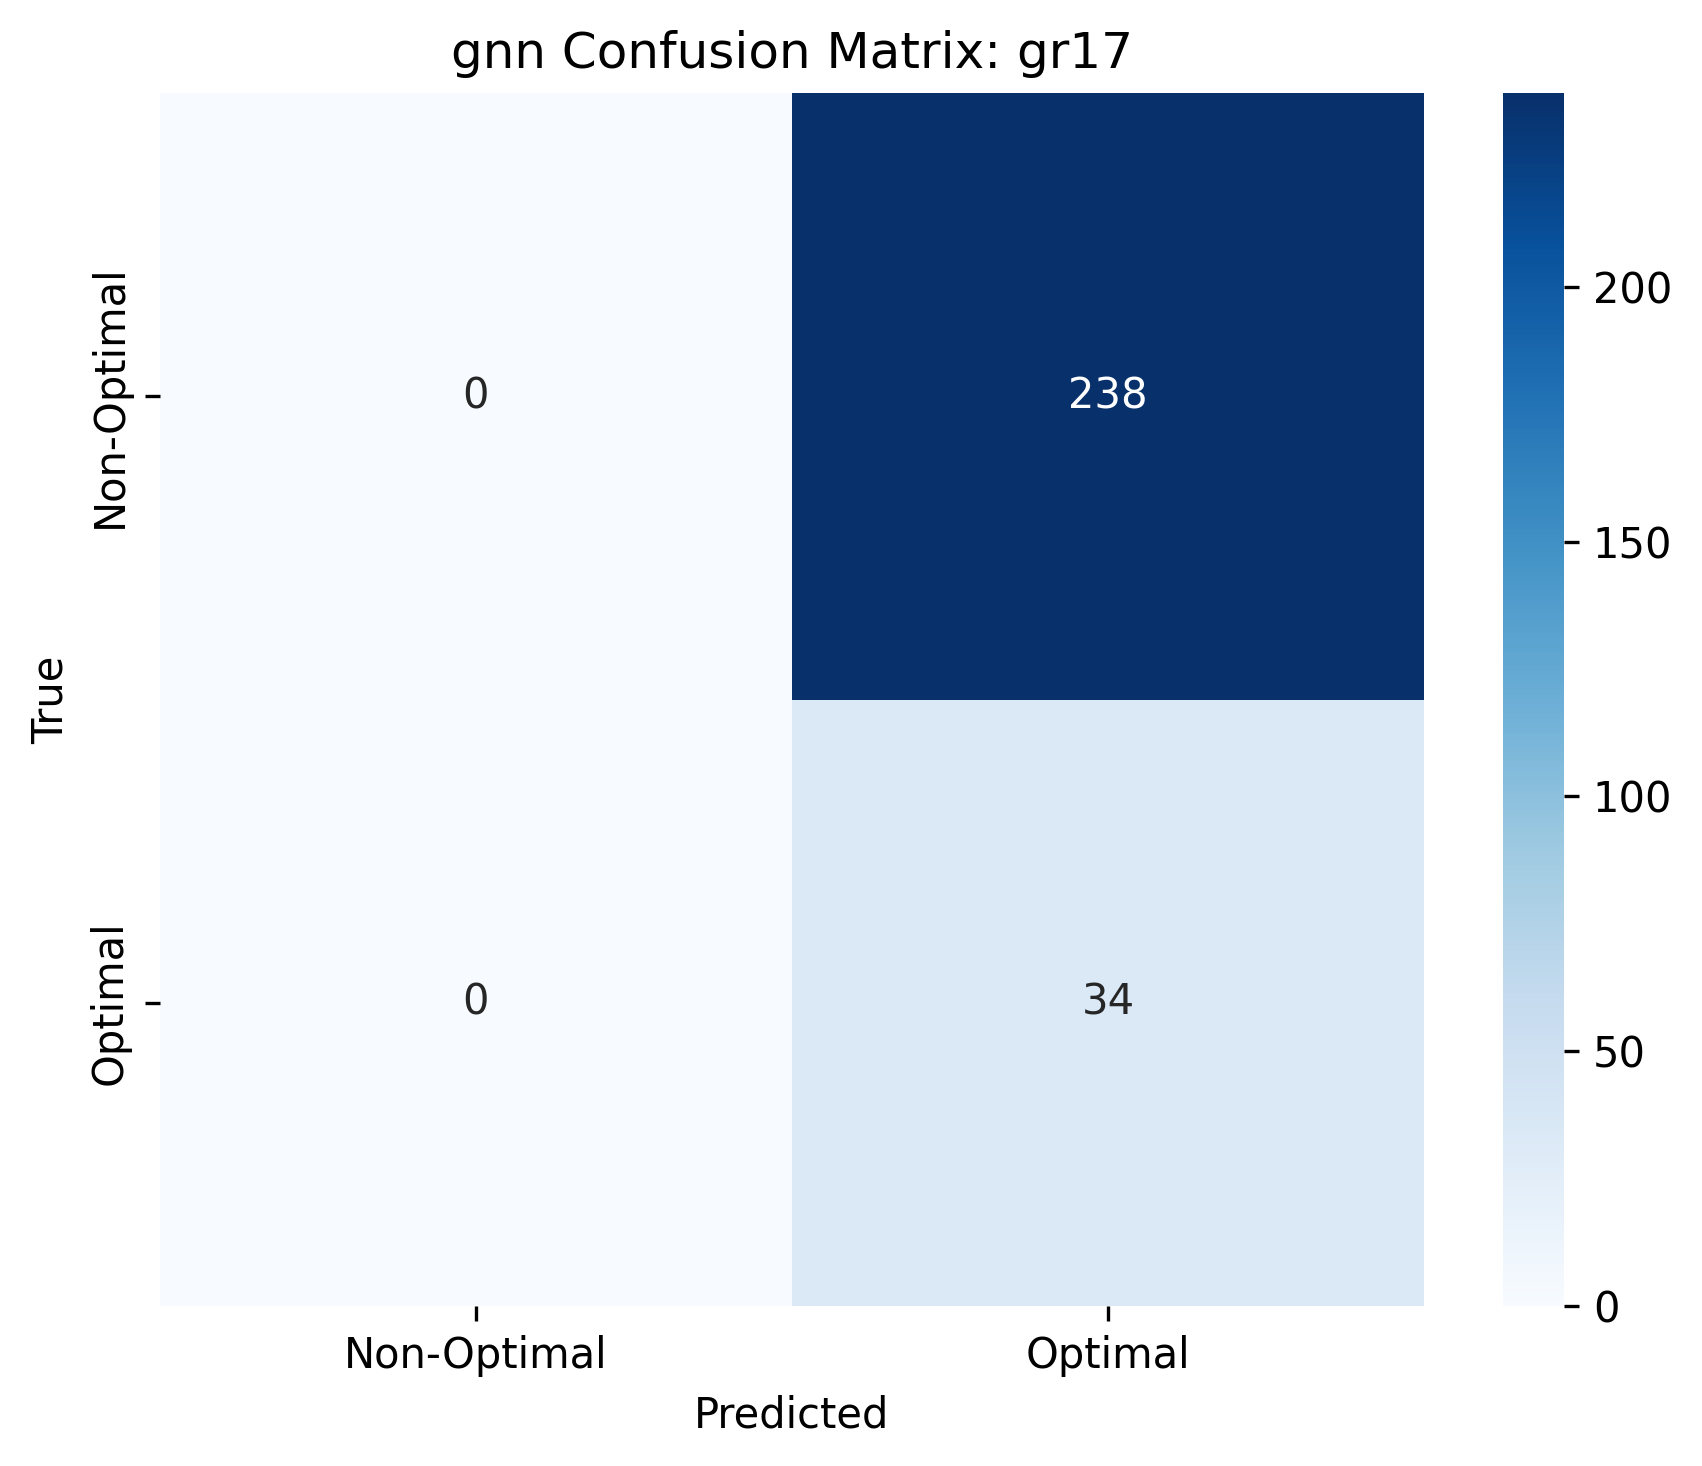
\includegraphics[width=0.32\textwidth]{figures/gr17_gnn_confusion_matrix}
		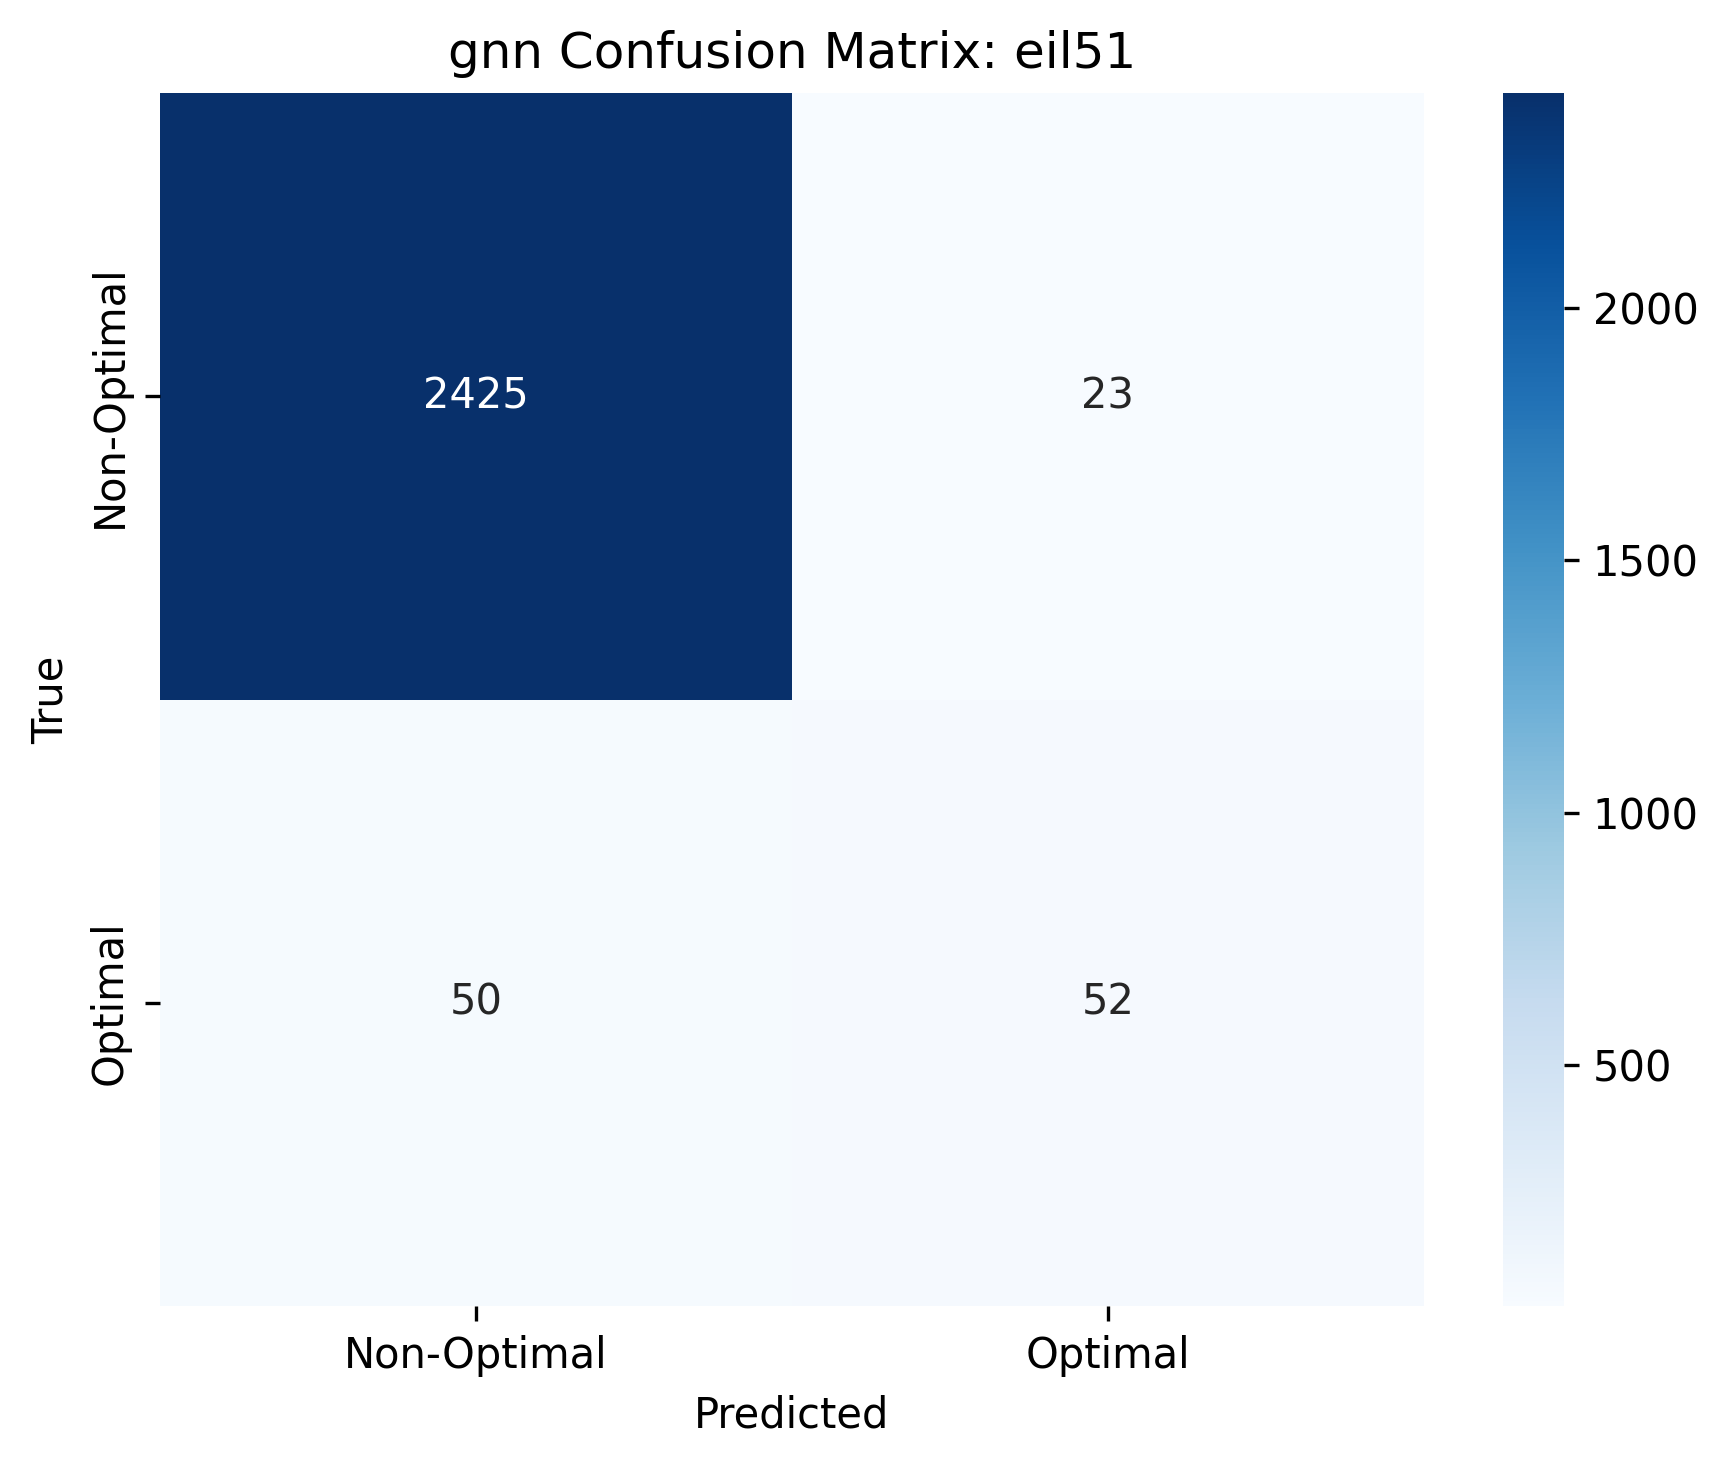
\includegraphics[width=0.32\textwidth]{figures/eil51_gnn_confusion_matrix}
		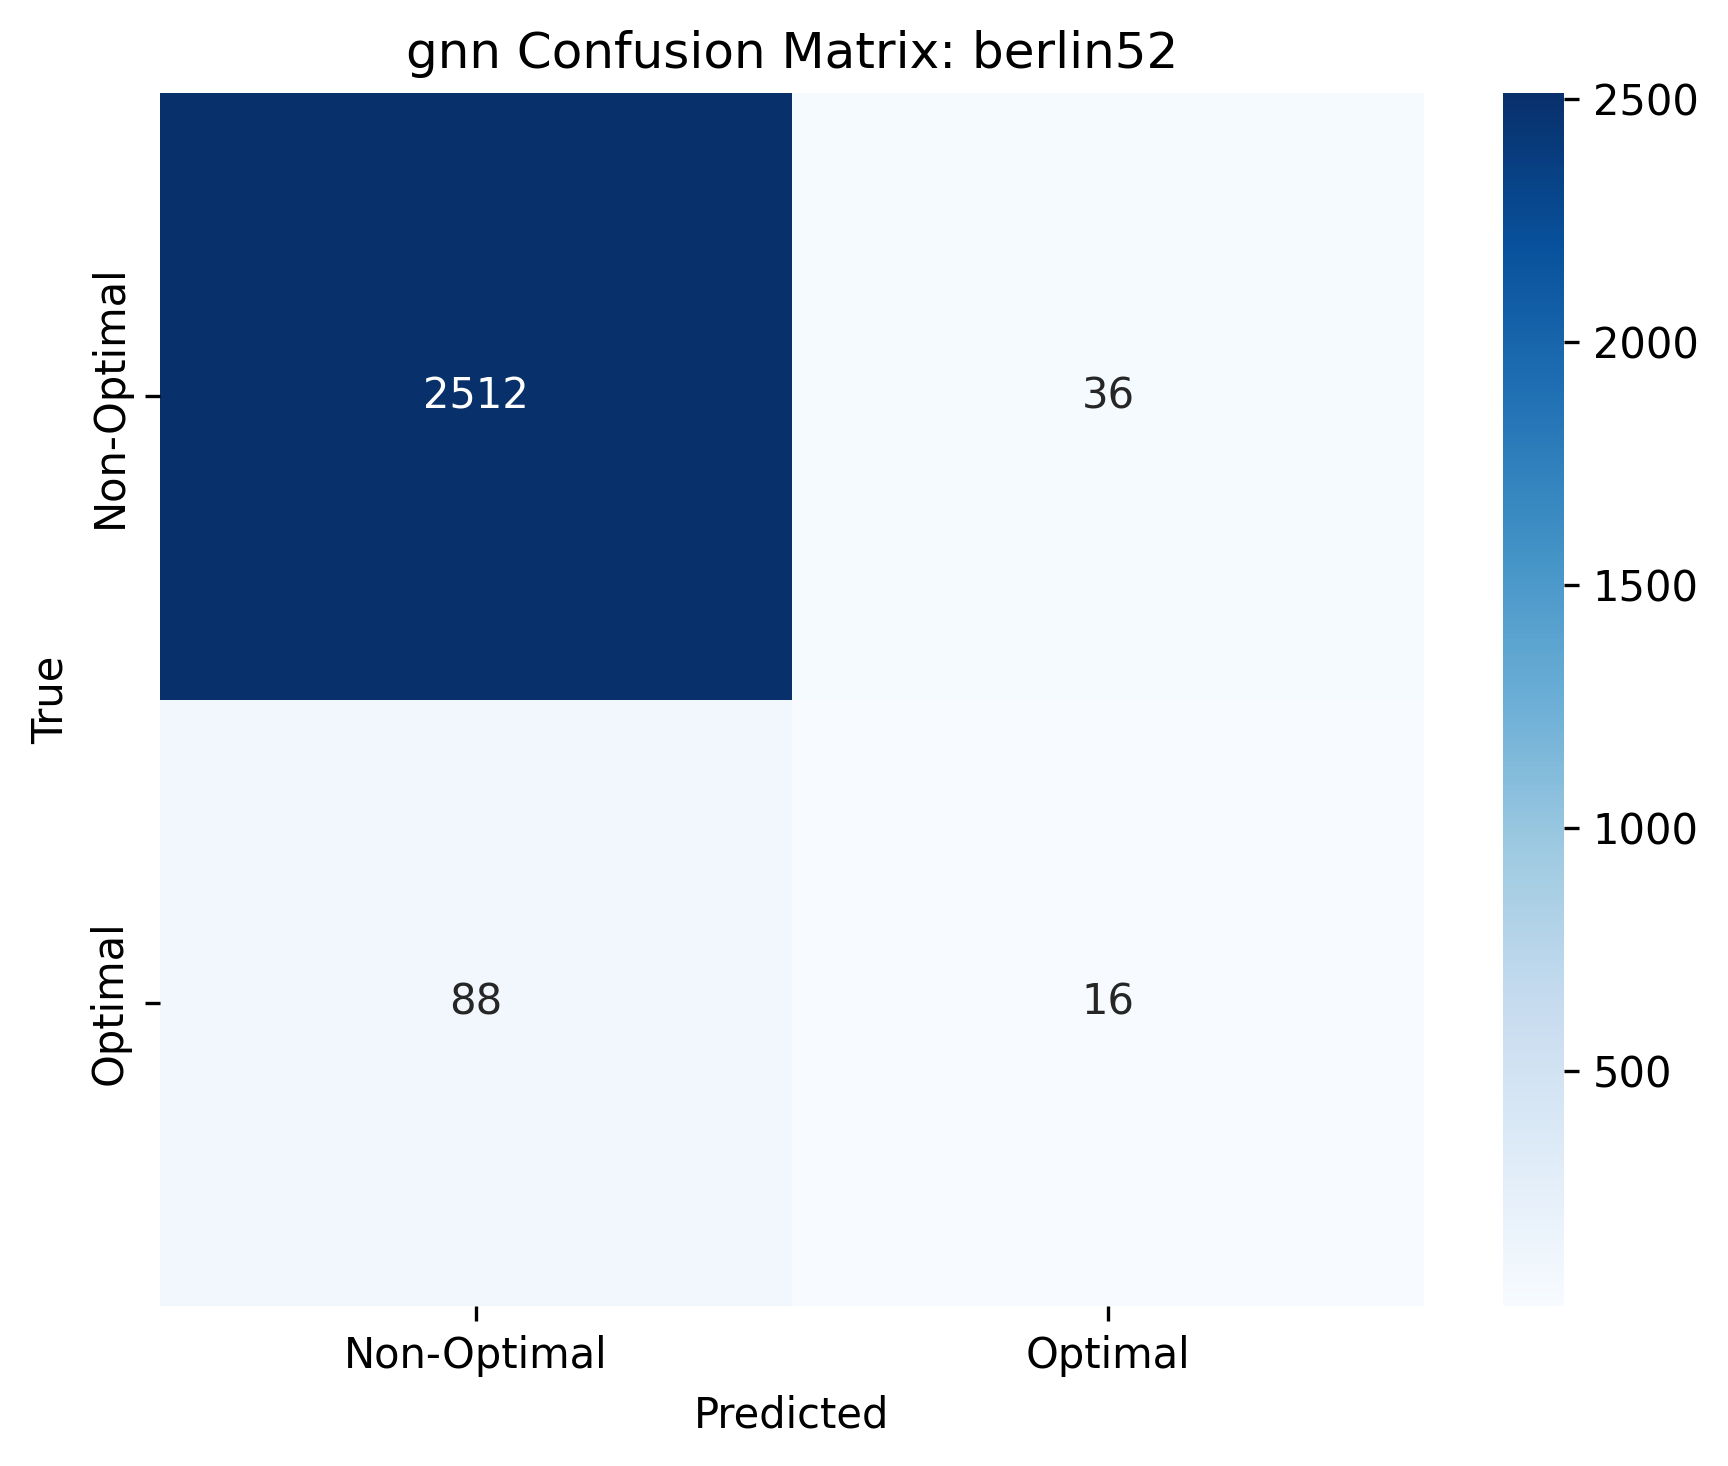
\includegraphics[width=0.32\textwidth]{figures/berlin52_gnn_confusion_matrix}\\[0.3em]
		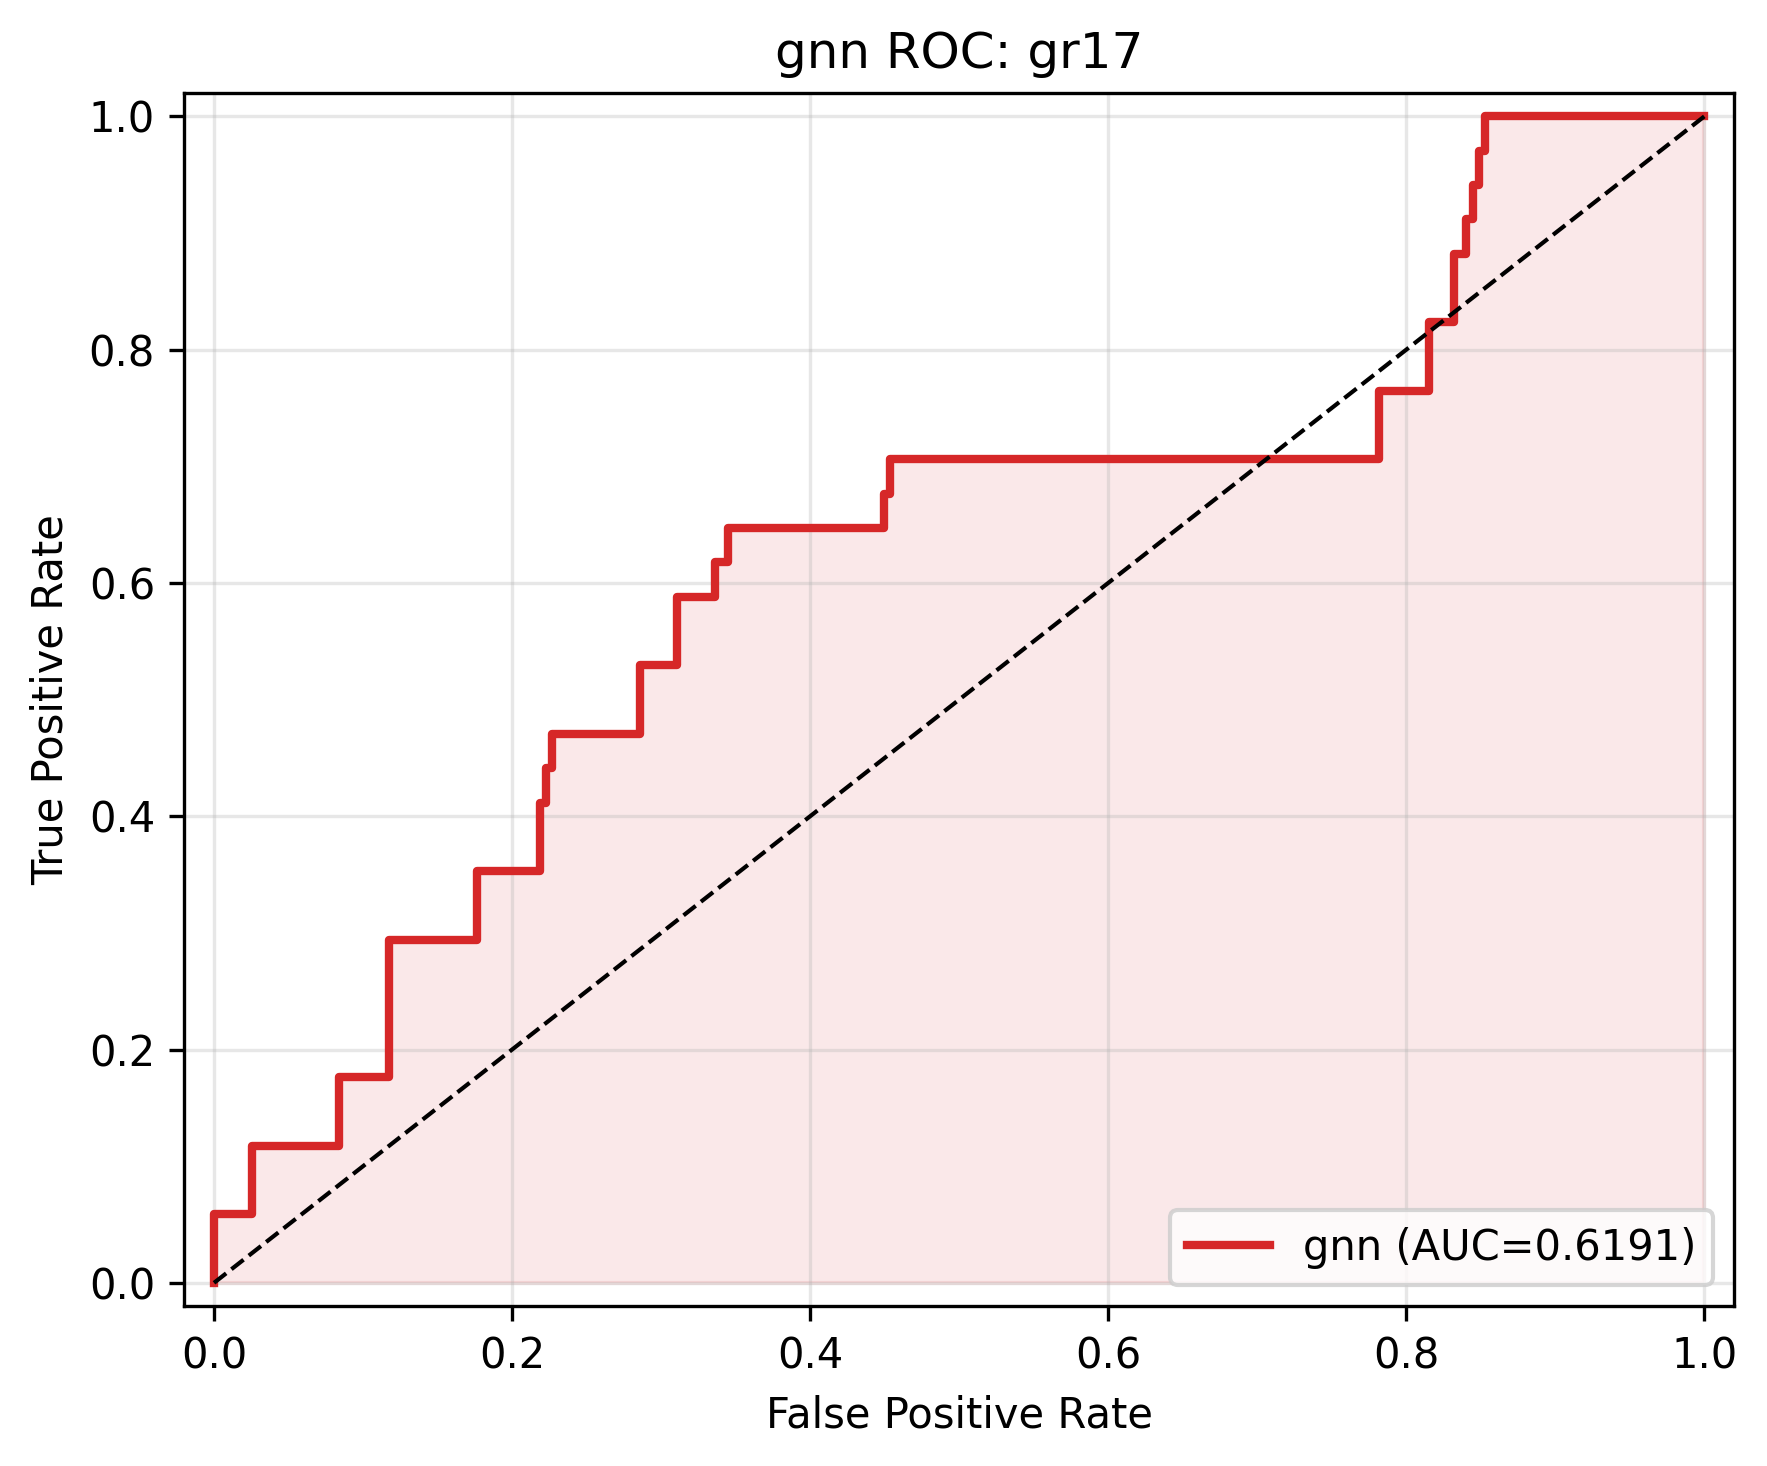
\includegraphics[width=0.32\textwidth]{figures/gr17_gnn_roc_auc}
		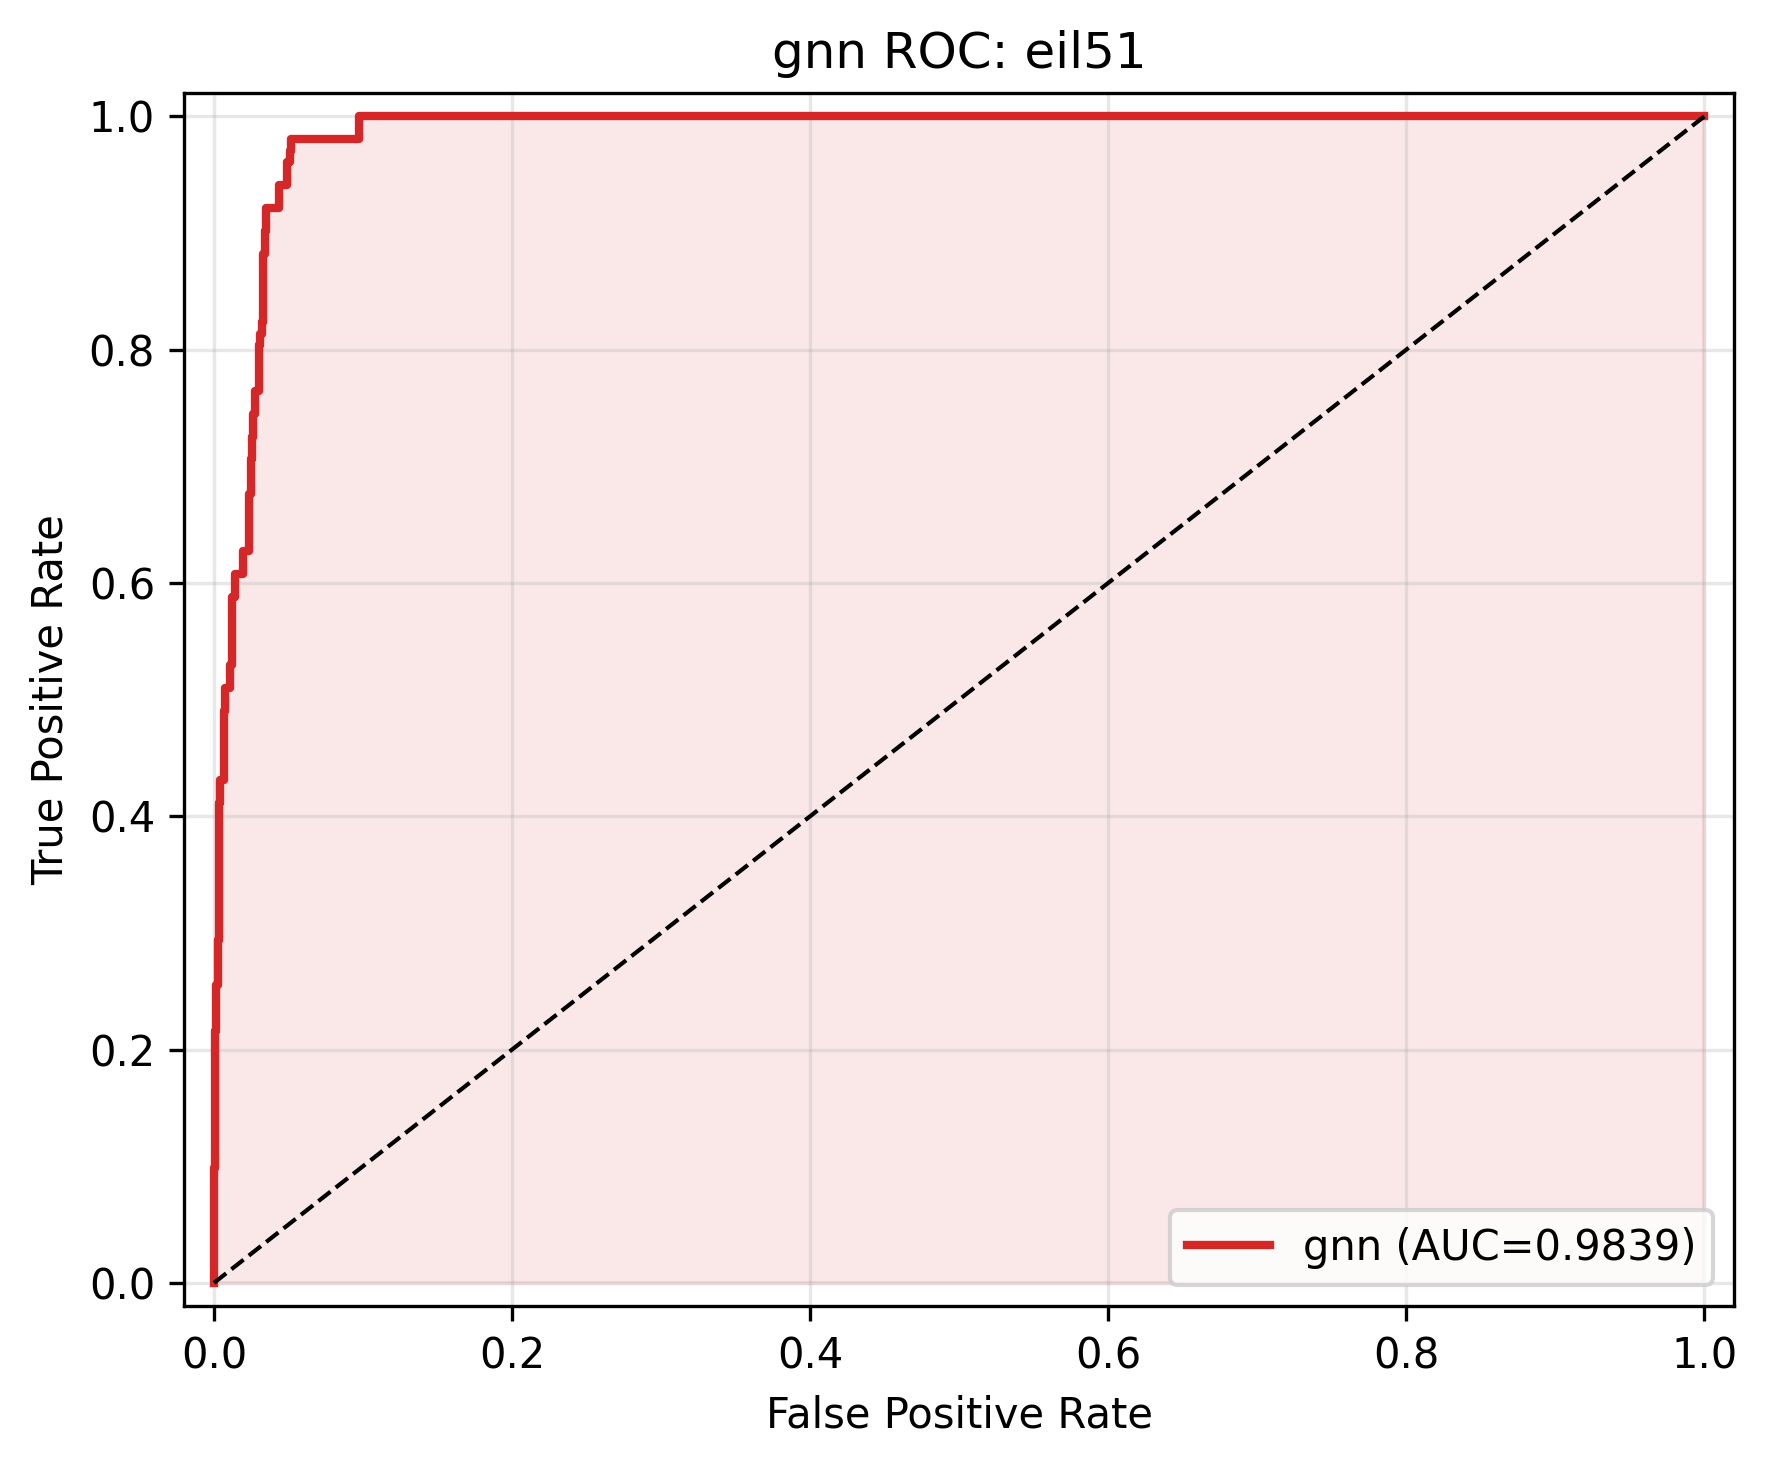
\includegraphics[width=0.32\textwidth]{figures/eil51_gnn_roc_auc}
		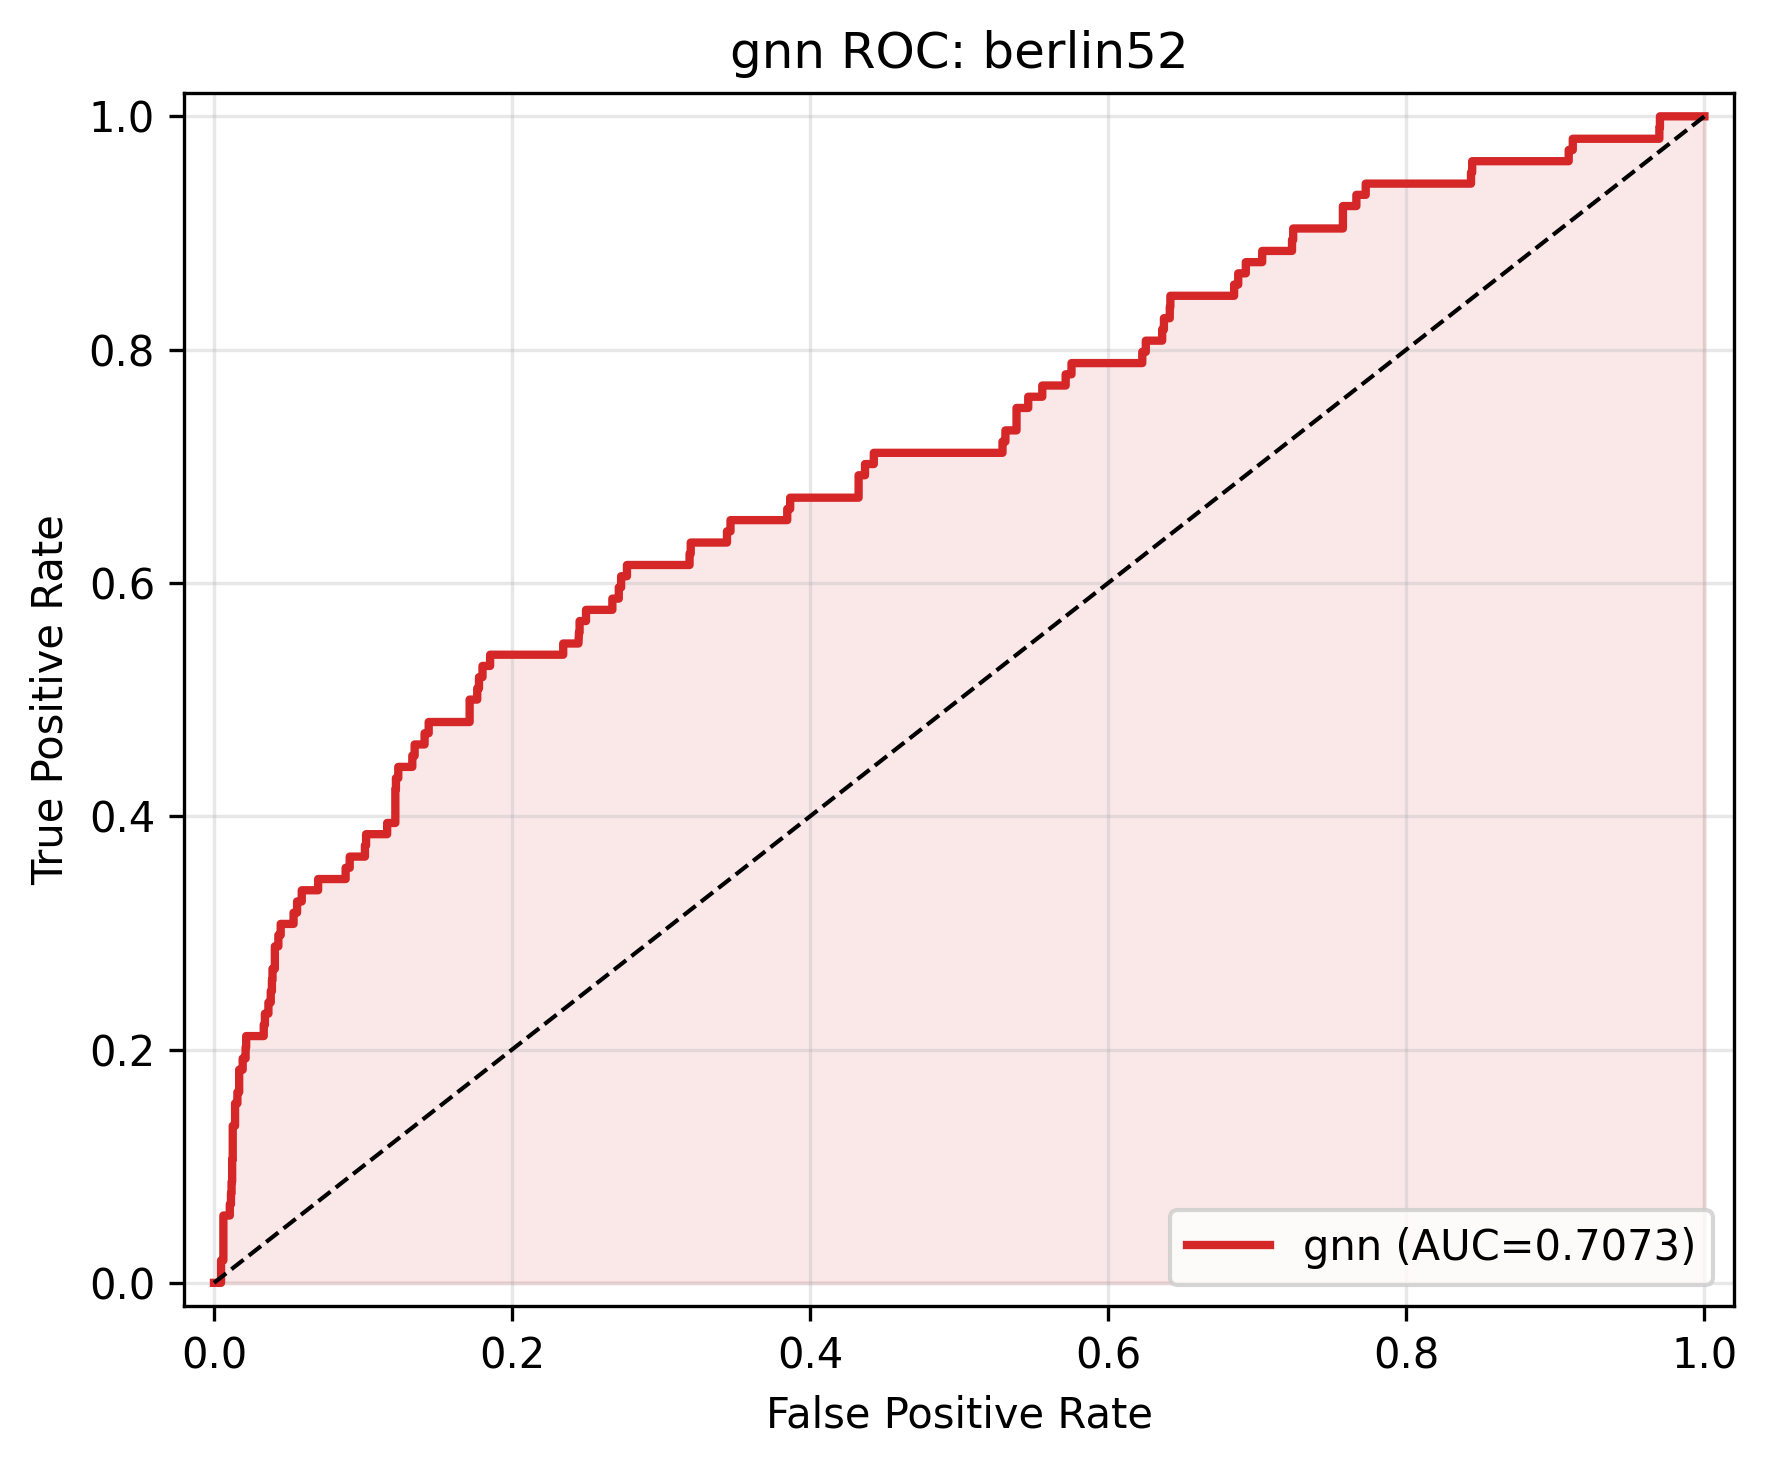
\includegraphics[width=0.32\textwidth]{figures/berlin52_gnn_roc_auc}
		\caption{Edge classification performance across three TSPLIB benchmarks by GNN.}
		\label{fig:gnn_evaluation}
	\end{figure}
	%Top row displays confusion matrices showing true/false positive/negative counts for optimal edge prediction. Bottom row presents ROC curves with AUC scores demonstrating superior ranking quality through message passing over graph topology.

	

	\begin{figure}[htbp]
		\centering
		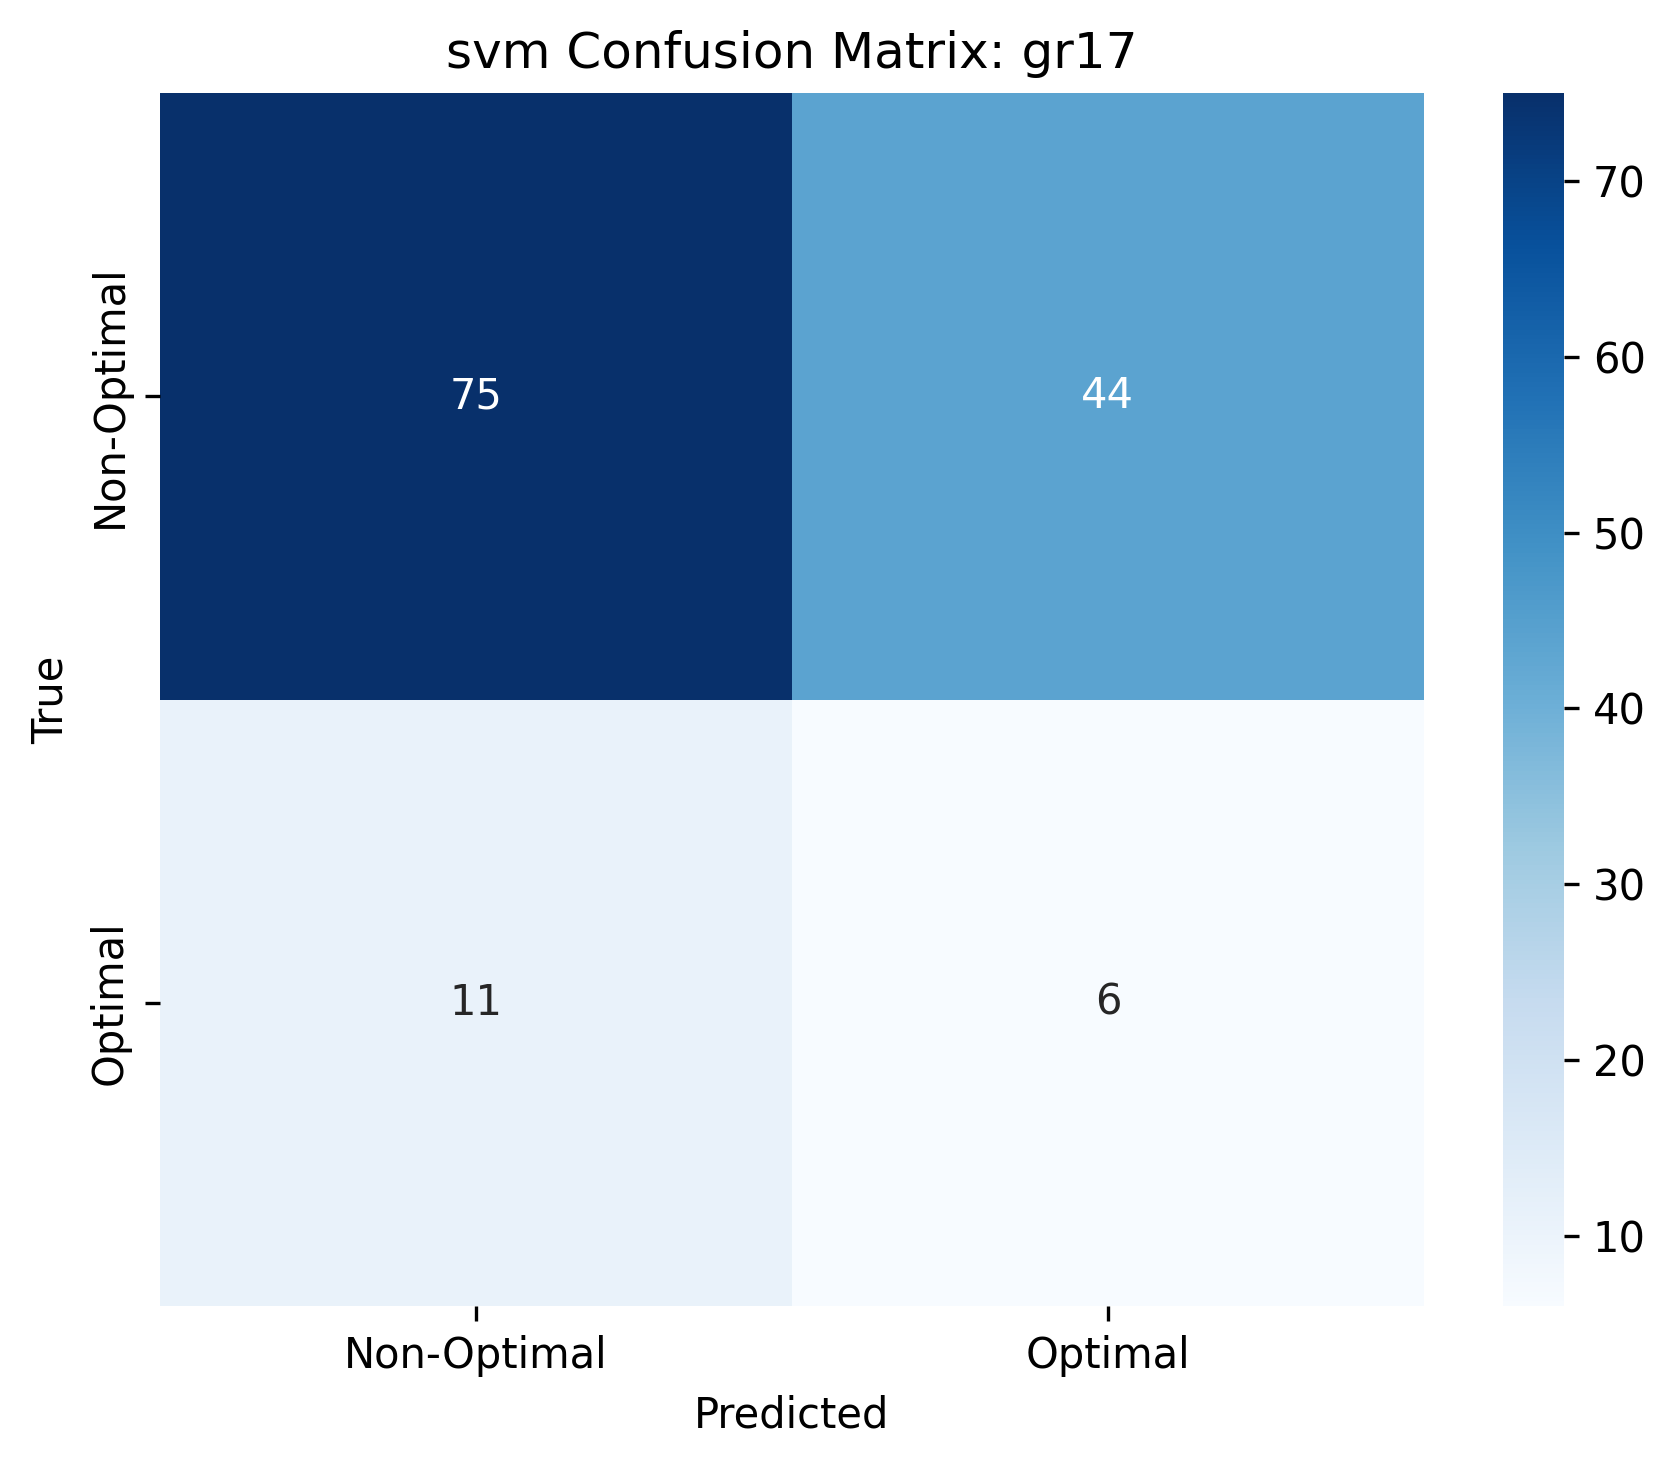
\includegraphics[width=0.32\textwidth]{figures/gr17_svm_confusion_matrix}
		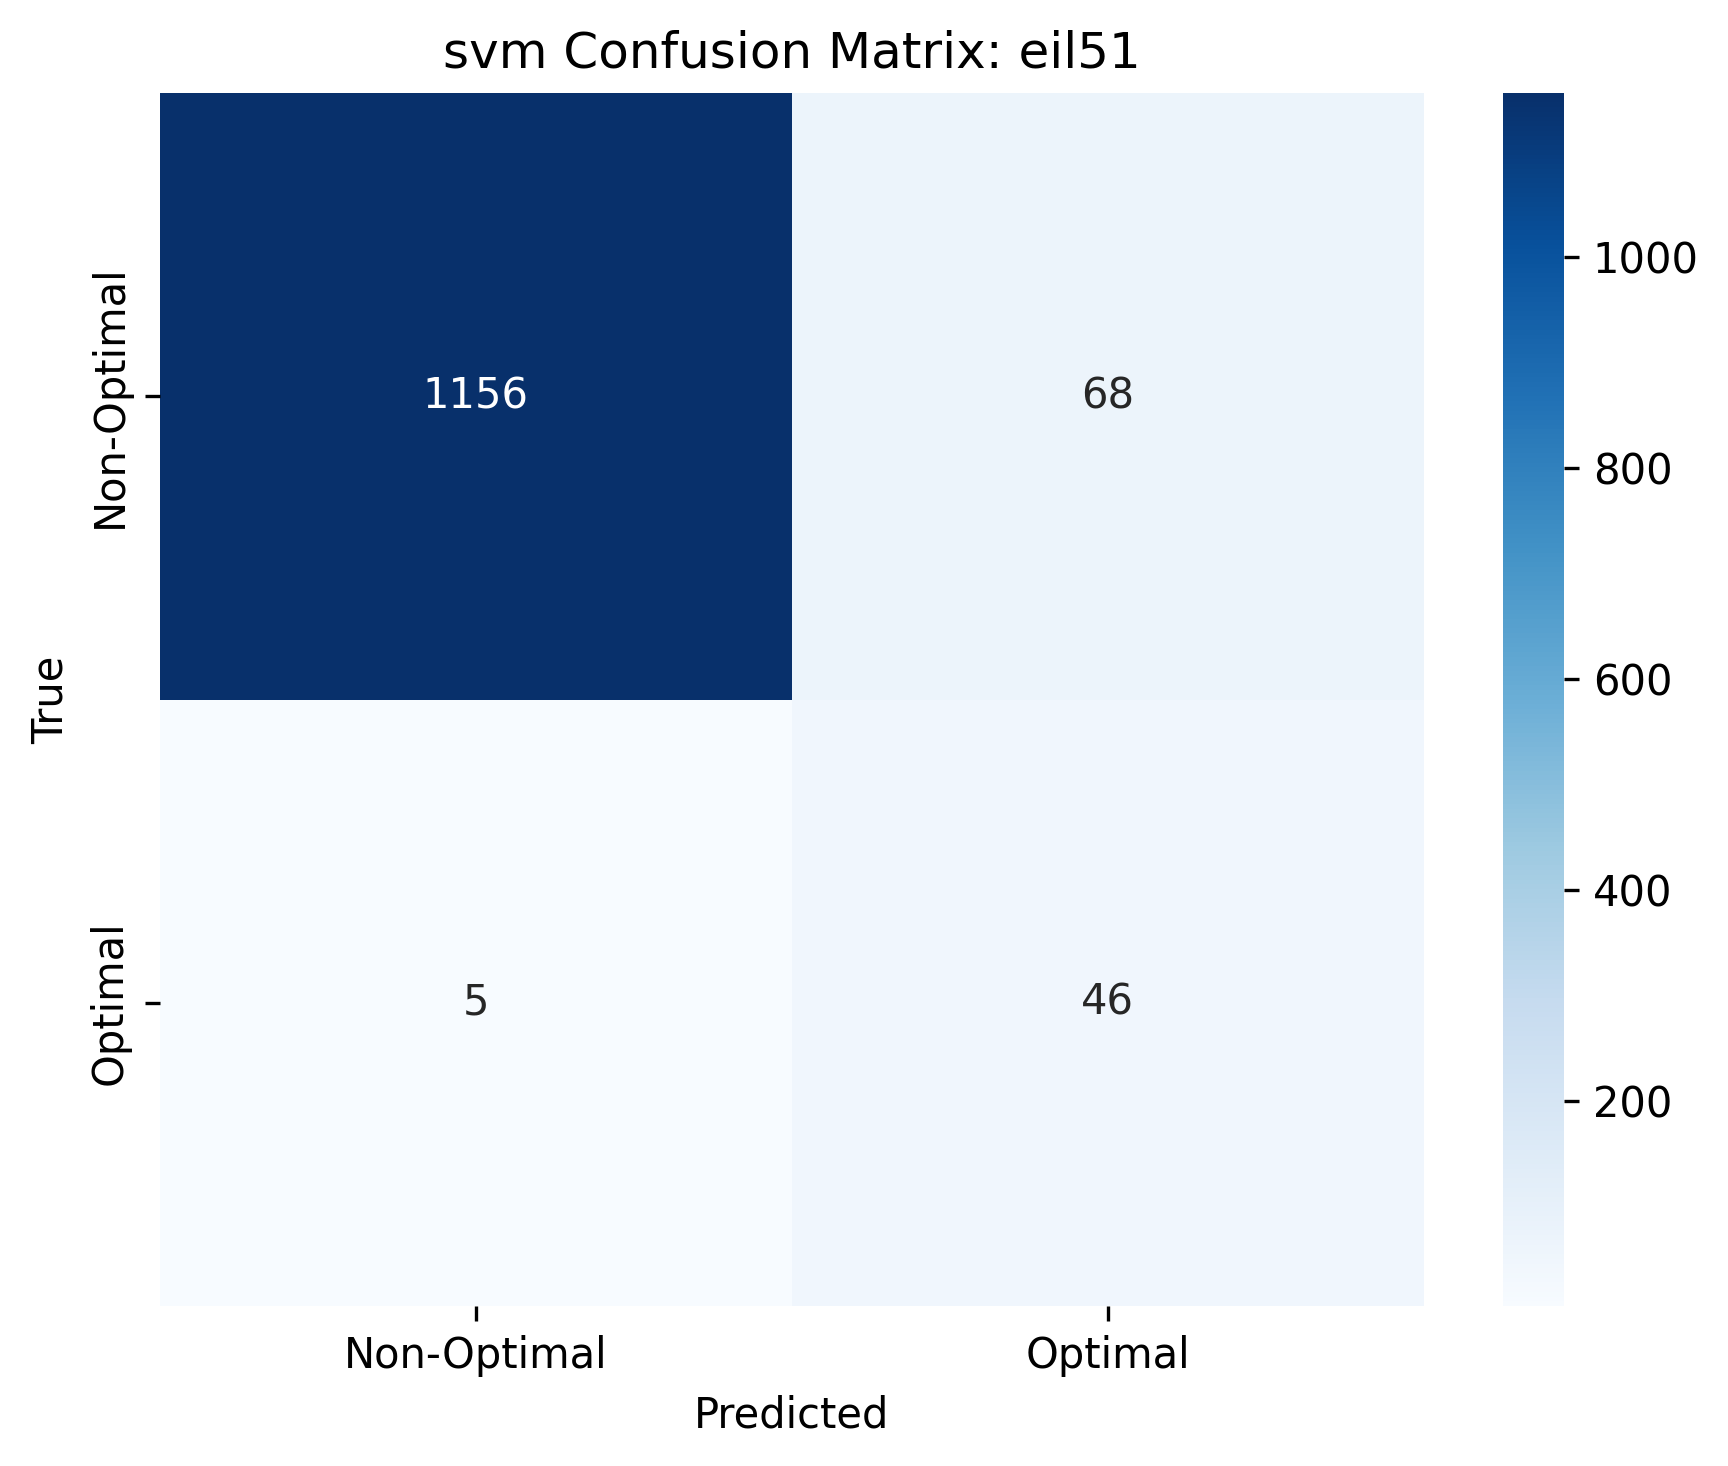
\includegraphics[width=0.32\textwidth]{figures/eil51_svm_confusion_matrix}
		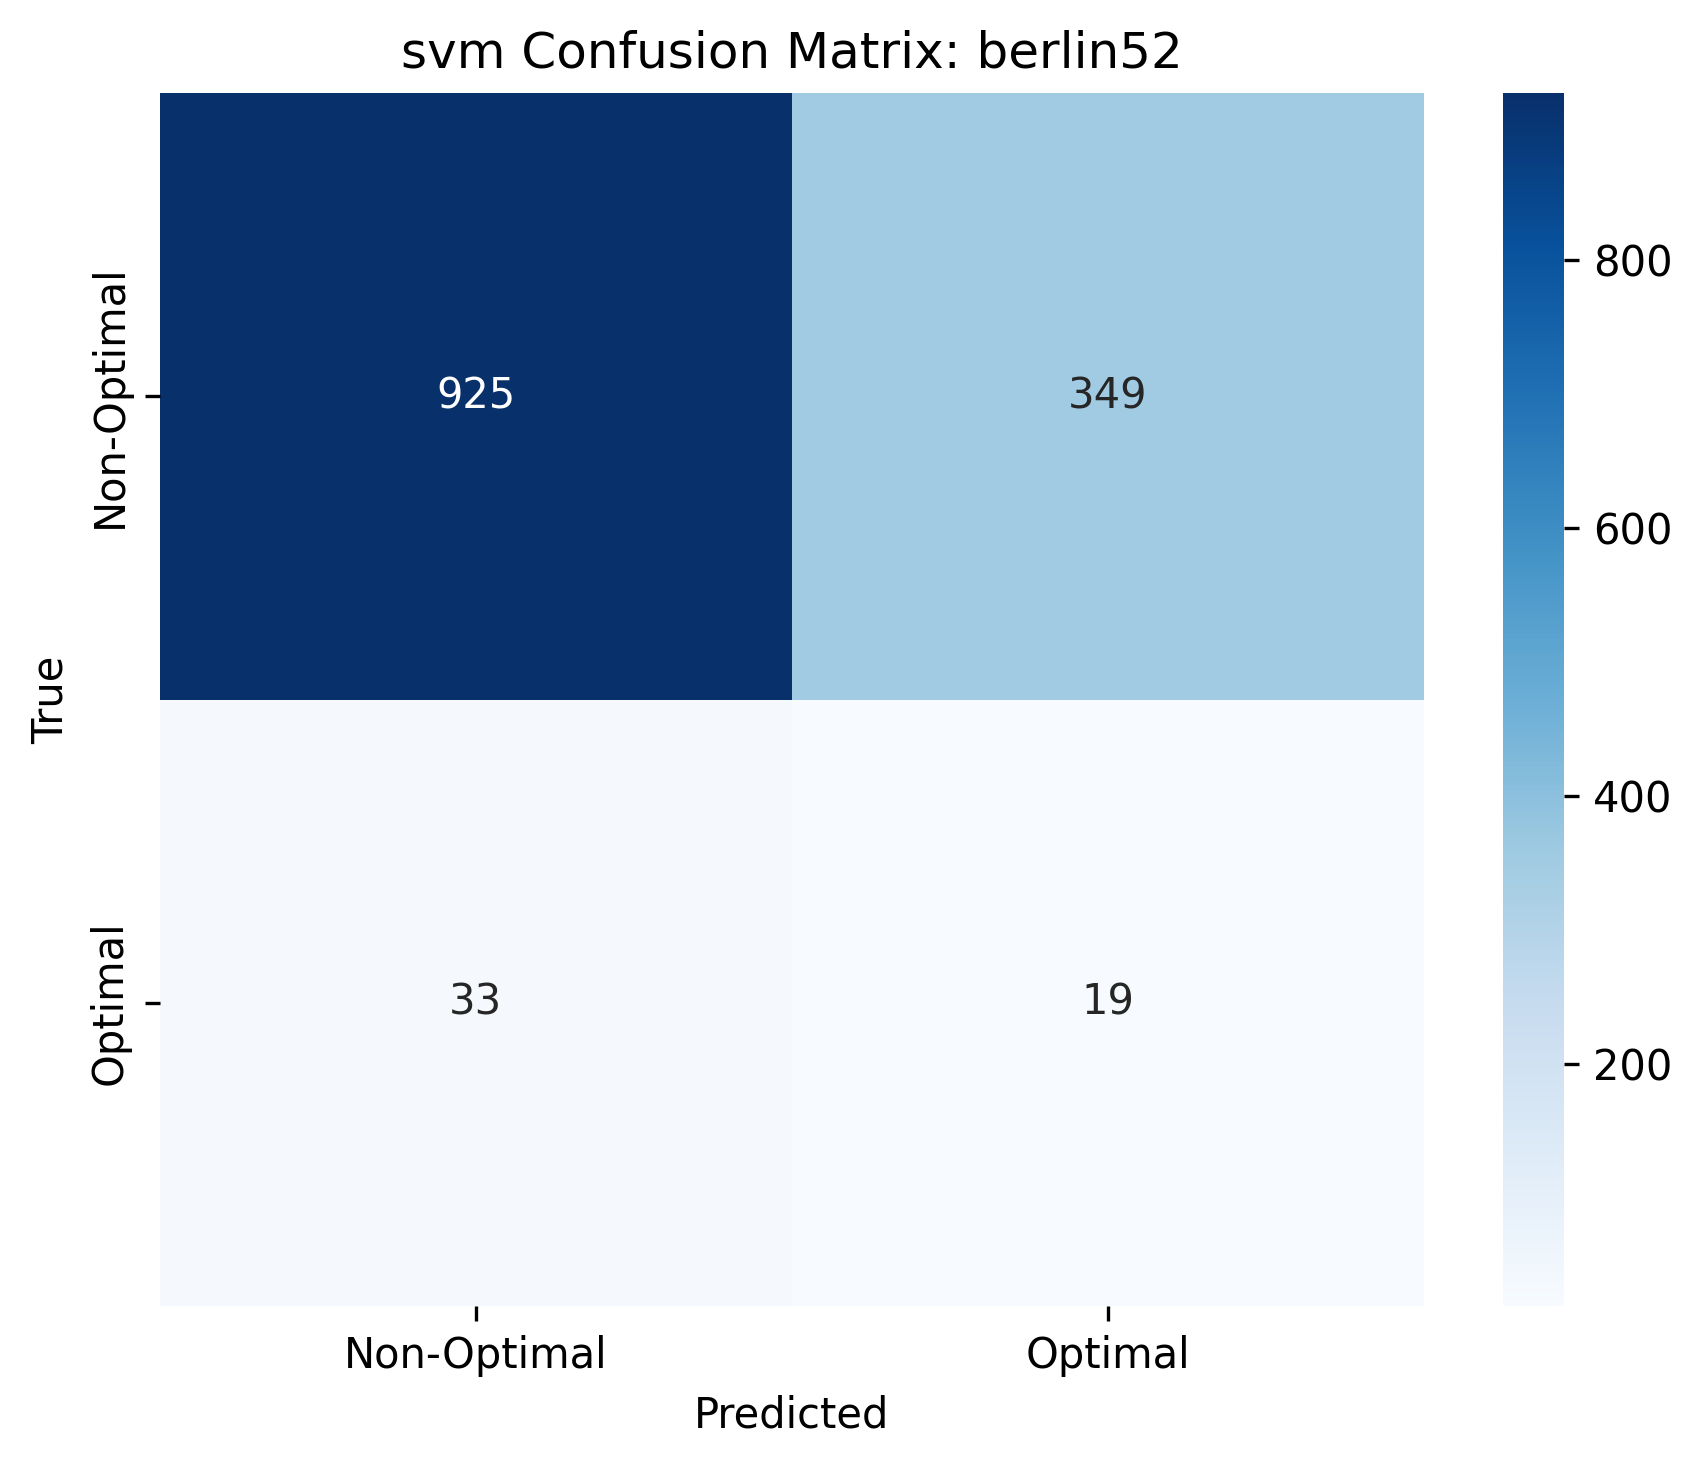
\includegraphics[width=0.32\textwidth]{figures/berlin52_svm_confusion_matrix}\\[0.3em]
		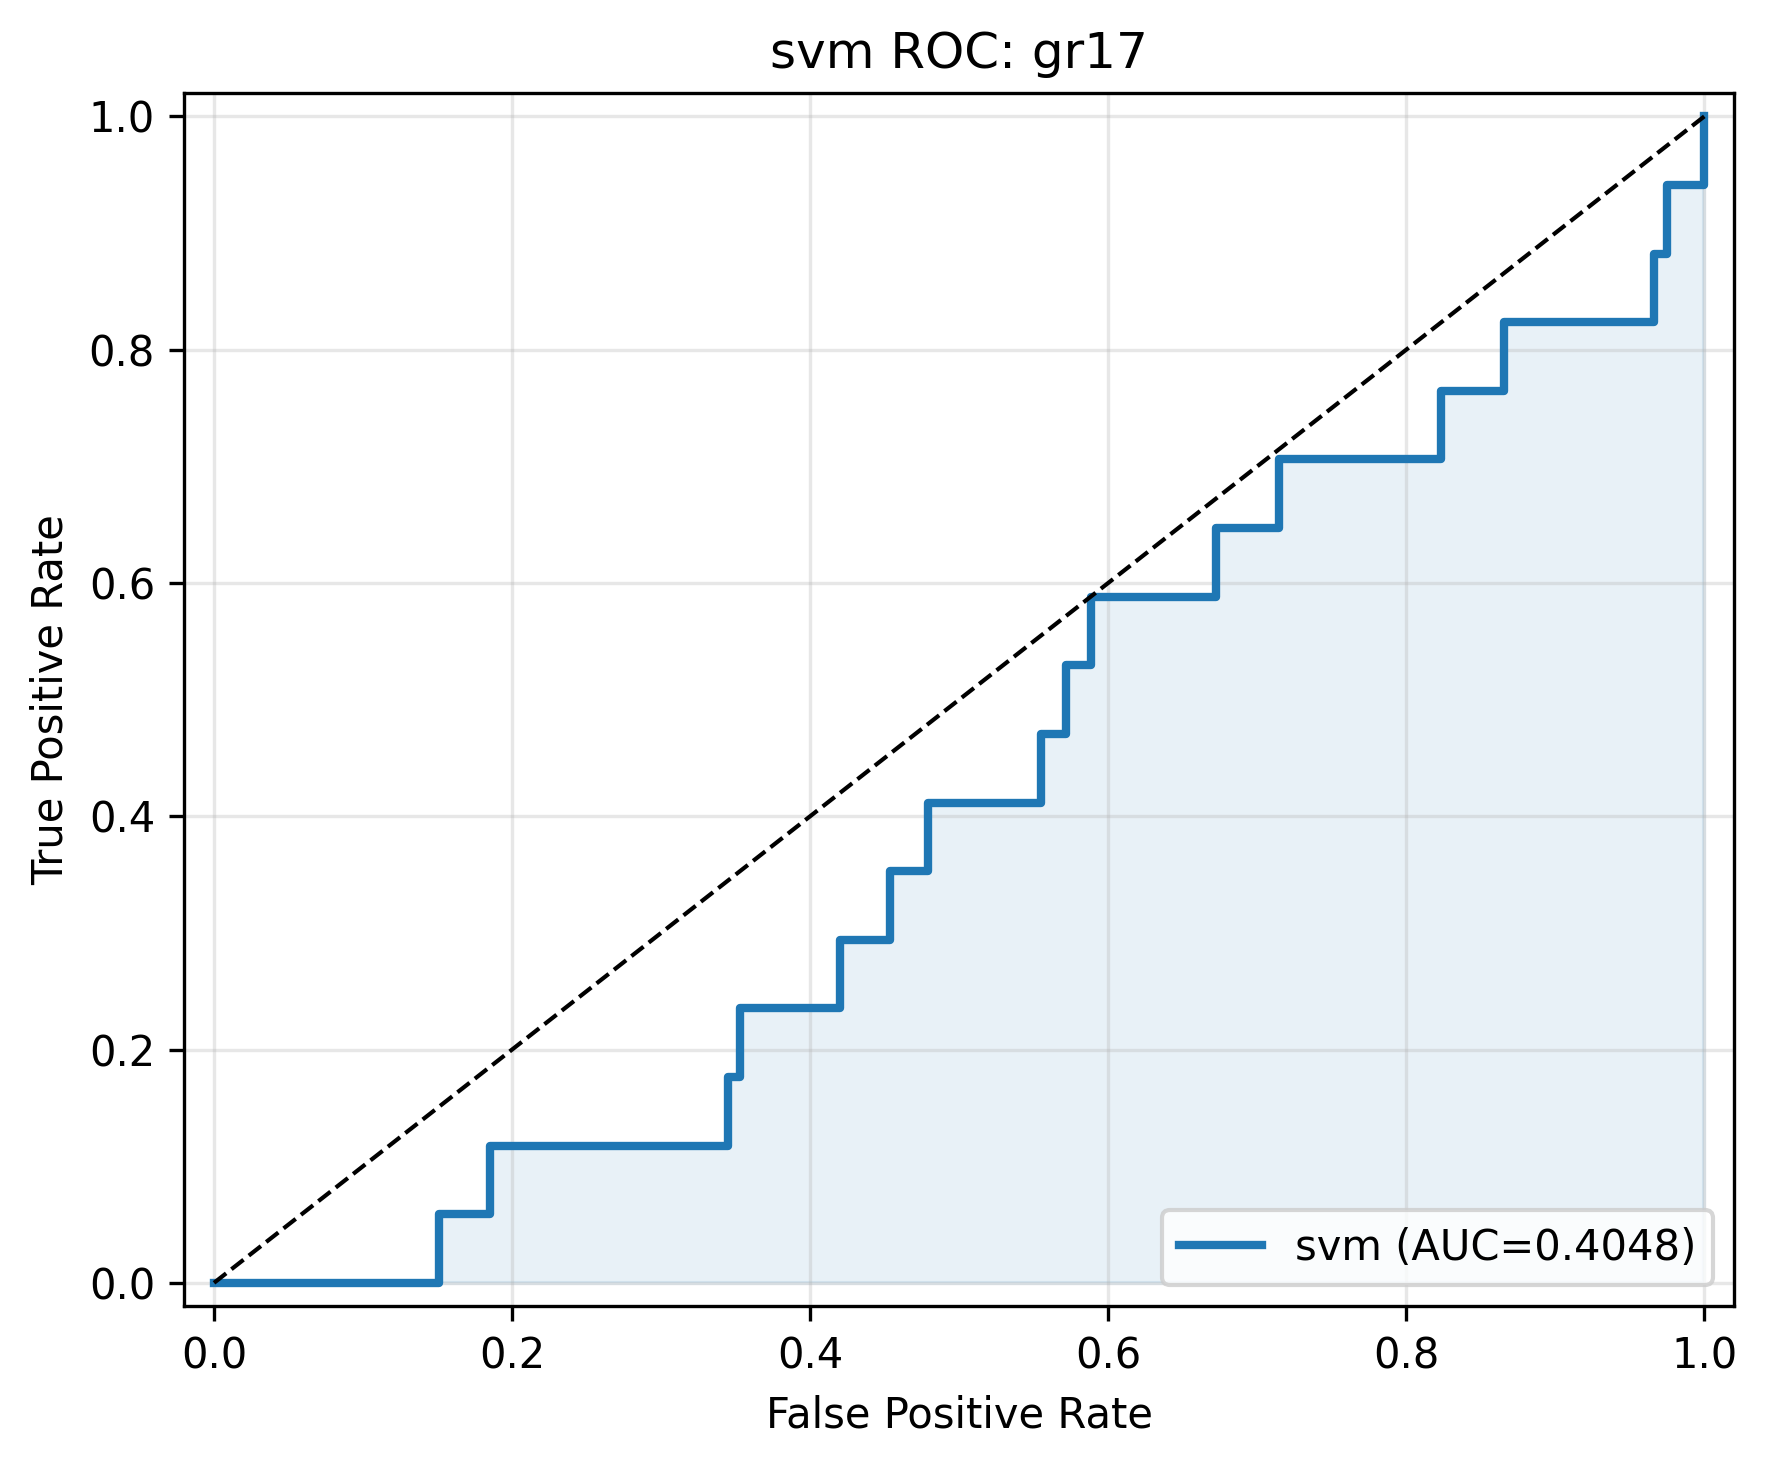
\includegraphics[width=0.32\textwidth]{figures/gr17_svm_roc_auc}
		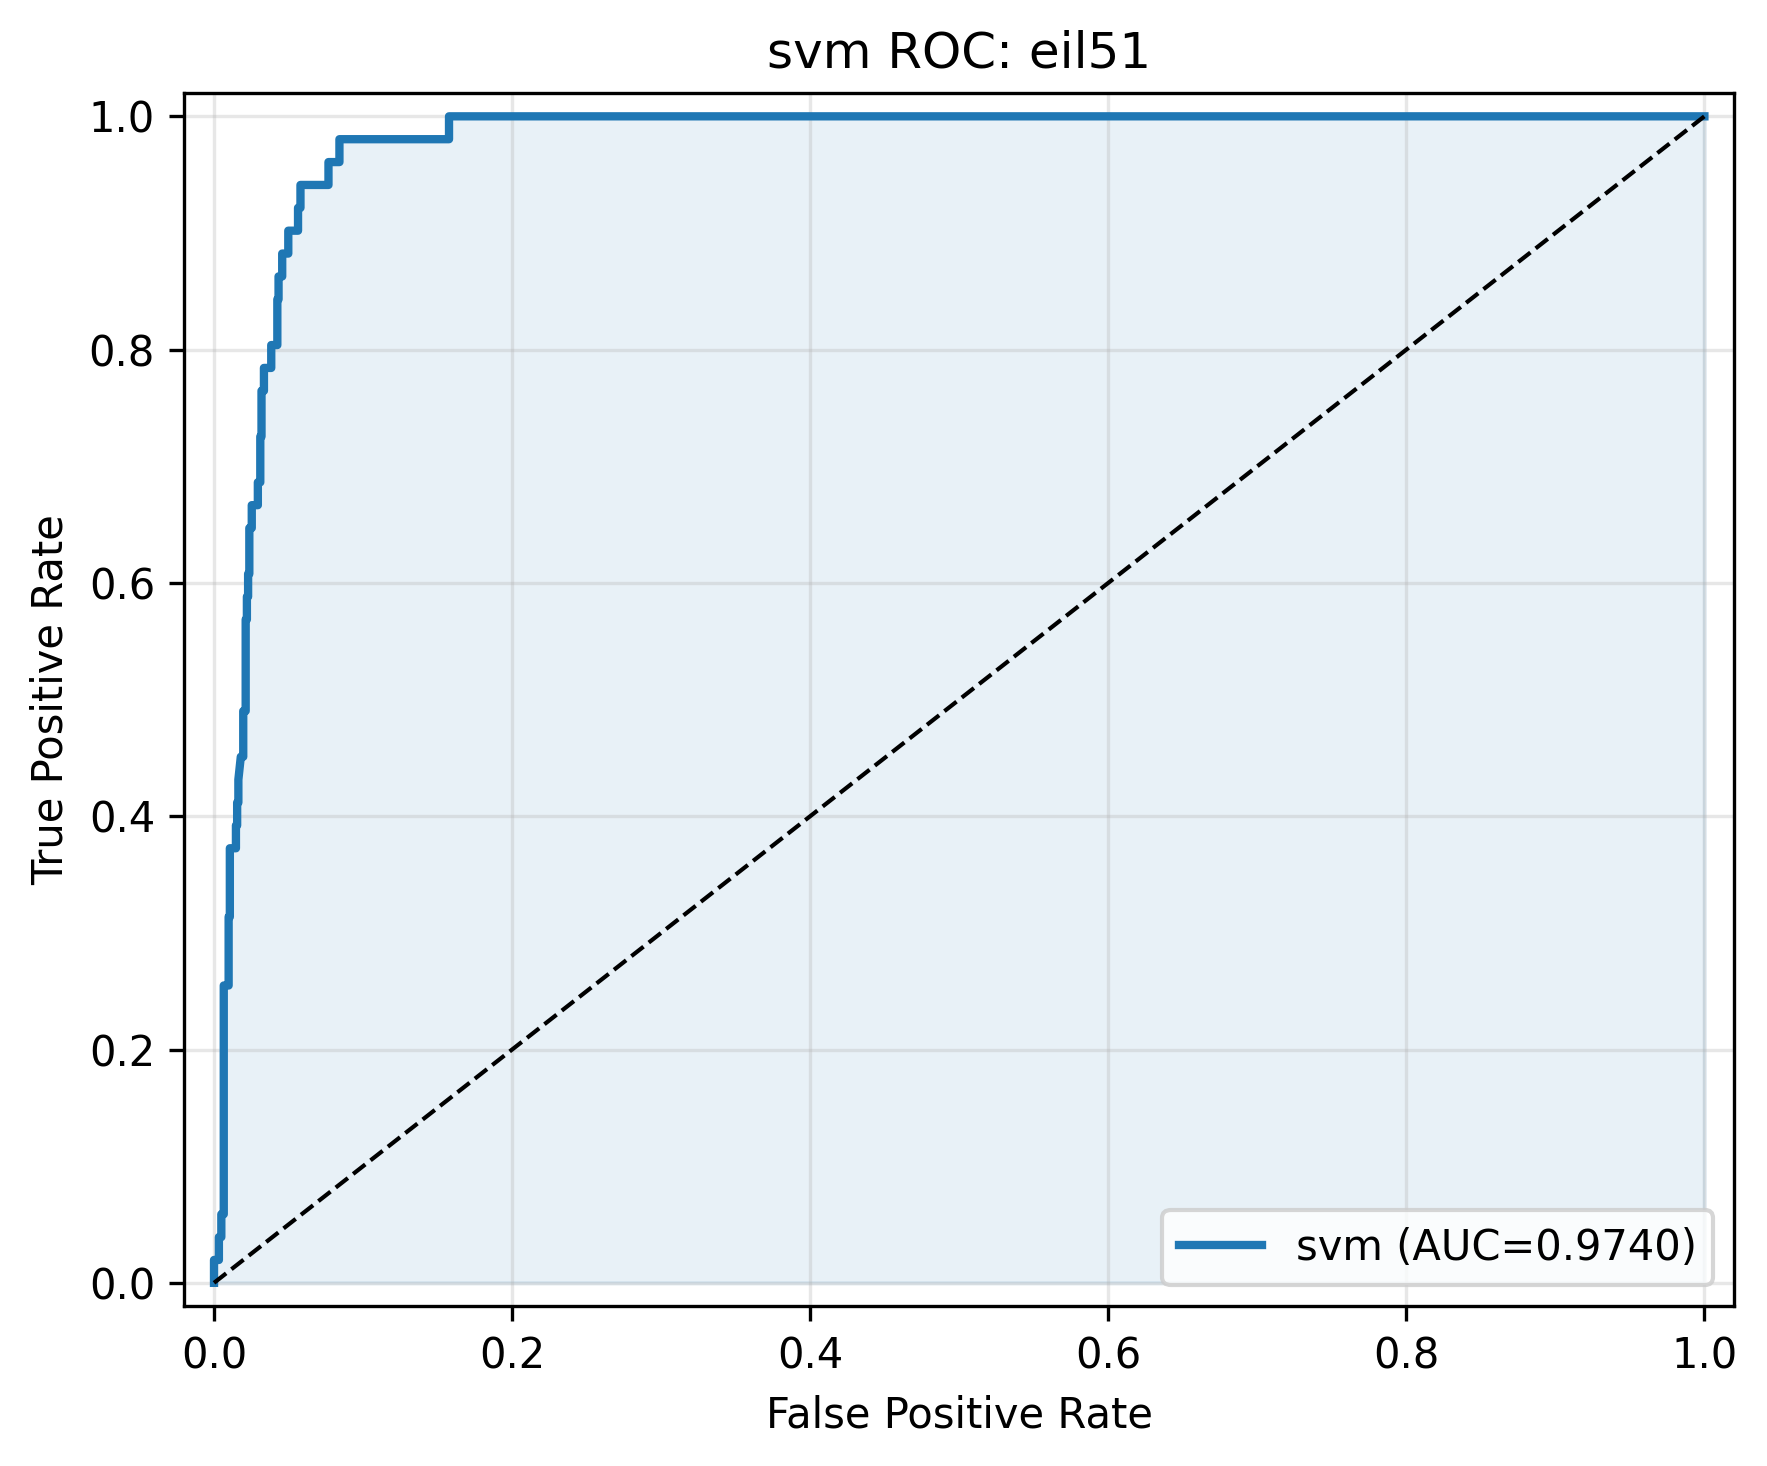
\includegraphics[width=0.32\textwidth]{figures/eil51_svm_roc_auc}
		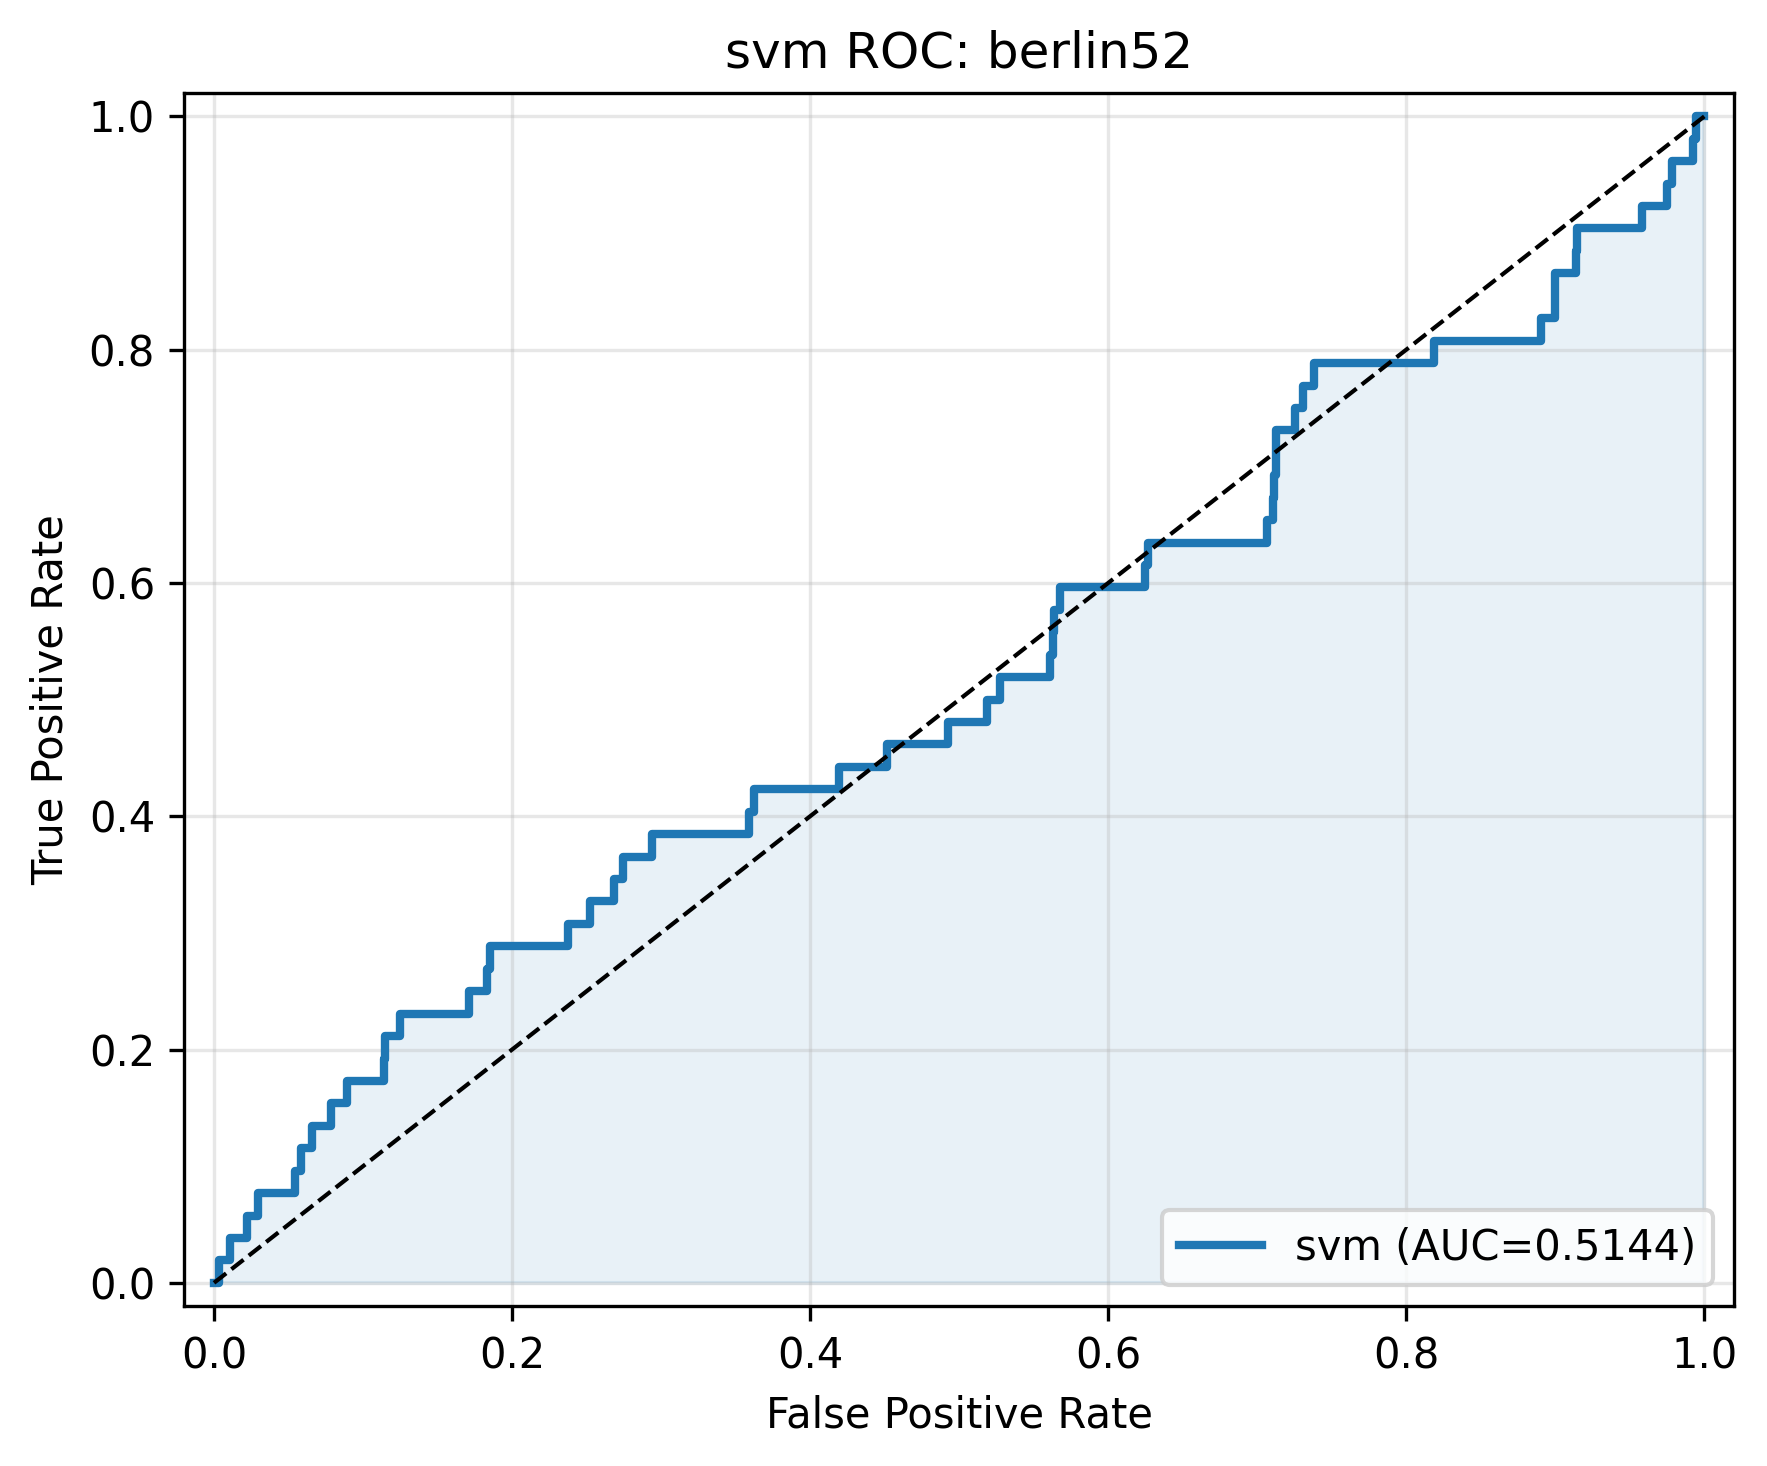
\includegraphics[width=0.32\textwidth]{figures/berlin52_svm_roc_auc}
		\caption{Edge classification performance across three TSPLIB benchmarks by SVM.}
		\label{fig:svm_evaluation}
	\end{figure}
	%Confusion matrices and ROC curves demonstrate that cost-sensitive SVM achieves high recall for optimal edges despite severe class imbalance, validating the statistical feature extraction pipeline.

	

	So, the sensitivity analysis of feature thresholds show f5 for gr17 and berlin52, and f2 for eil51, are the most important features, by the feature ablation and AUC and F1 values in the Table \ref{tab:feature_ablation_compact}. As shown in Table~\ref{tab:svm_vs_gnn_comparison} the GNN consistently outperforms the SVM across all instances. Notably, the optimal scaling factors differ between models, with the GNN requiring lower scaling (5-10) compared to the SVM's optimal $\tau$ (10-25), suggesting that the GNN's expressive power compensates for the need for aggressive class-weighting. Positive ratio indicates the proportion of optimal edges in each instance. SVM optimal $\tau$ and GNN optimal scaling were determined by maximizing F1 score.
	%with the most significant improvement observed on gr17 (AUC: 0.8234 vs 0.4684) and berlin52 (AUC: 0.7123 vs 0.6167). For the larger instances (eil51 and berlin52), the GNN achieves near-perfect performance with $AUC > 0.98$ for eil51. 

	

	\begin{table}[htbp]
		\centering
		\caption{Feature Ablation Results: AUC Drop When Each Feature is Removed}
		\label{tab:feature_ablation_compact}
		\begin{tabular}{l|cc|cc|cc} \hline
		Feature & \multicolumn{2}{c}{gr17} & \multicolumn{2}{c}{eil51} & \multicolumn{2}{c}{berlin52} \\ \hline
			& {AUC Drop} & {F1 Drop} & {AUC Drop} & {F1 Drop} & {AUC Drop} & {F1 Drop} \\ \hline
			f1 & 0.0270 & -0.0074 & 0.0007 & 0.0040 & 0.0116 & 0.0113 \\
			f2 & 0.0194 & -0.0073 & \textbf{0.0048} & 0.0274 & -0.0211 & -0.0045 \\
			f3 & 0.0162 & -0.0224 & -0.0009 & 0.0067 & 0.0233 & 0.0035 \\
			f4 & -0.0039 & 0.0087 & -0.0018 & -0.0065 & -0.0367 & -0.0219 \\
			f5 & \textbf{0.0490} & -0.0250 & -0.0013 & 0.0082 & \textbf{0.0570} & 0.0124 \\
			f6 & -0.0194 & -0.0171 & -0.0050 & -0.0001 & -0.0779 & -0.0067 \\ \hline
			\end{tabular}
	\end{table}

	

	

	

	\begin{table}[htbp]
		\centering
		\caption{SVM and GNN Comparison}
		\label{tab:svm_vs_gnn_comparison}
		\begin{tabular}{l|cccccc}\hline
			Instance & Cities & \makecell{Positive \\ Ratio} & \makecell{SVM \\ Optimal $\tau$} & \makecell{GNN \\ Optimal Scaling} & \makecell{SVM \\ Best AUC} & \makecell{GNN \\ Best AUC} \\ \hline
			gr17     & 17  & 0.125 & 25 & 5  & 0.4684 & 0.8234 \\
			eil51    & 51  & 0.040 & 10 & 10 & 0.9770 & 0.9856 \\
			berlin52 & 52  & 0.039 & 25 & 5  & 0.6167 & 0.7123 \\ \hline
		\end{tabular}
	\end{table}

	

	

	\section{Conclusion}
	 This manuscript has detailed a unified methodological framework that bridges classical statistical problem reduction with modern topology-aware deep learning, demonstrating that both paradigms achieve complementary strengths in optimality preservation and computational efficiency. Experimental results across three benchmark instances confirm that sampling-based statistical features provide robust edge relevance signals, while graph neural networks consistently outperform independent classifiers by leveraging message passing to capture structural dependencies. Future work will focus on integrating temporal graph dynamics with real-time multi-agent coordination and developing verifiable deployment pipelines that guarantee suboptimality bounds under distributional shift.

	

	\begin{thebibliography}{99}

		

		\bibitem[Applegate et al. (2006a)]{applegate2006traveling}
		Applegate D.L., Bixby R.E., Chvatal V. and Cook W.J. (2006), {\it The traveling salesman problem: a computational study}, Princeton University Press.

		

		\bibitem[Applegate et al. (2006b)]{applegate2006concorde}
		Applegate D., Bixby R., Chv\'atal V. and Cook W. (2006), Concorde {TSP} solver, \url{http://www.math.uwaterloo.ca/tsp/concorde/}.

		

		\bibitem[Berry (1941)]{Berry1941}
		Berry A.C. (1941), The accuracy of the Gaussian approximation to the sum of independent variates, {\it Transactions of the american mathematical society}, 49(1), 122--136.

		

		\bibitem[Korolev and Shevtsova (2010)]{Korolev2010}
		Korolev V.Y. and Shevtsova I.G. (2010), On the upper bound for the absolute constant in the Berry–Esseen inequality, {\it Theory of Probability \& Its Applications}, 54(4), 638--658.

								

		\bibitem[Li et al. (2018)]{li2018combinatorial}
		Li Z., Chen Q. and Koltun V. (2018), Combinatorial optimization with graph convolutional networks and guided tree search, {\it Advances in Neural Information Processing Systems} 539--548.

		

		\bibitem[Lin and Kernighan (1973)]{lin1973effective}
		Lin S. and Kernighan B.W. (1973), An effective heuristic algorithm for the traveling-salesman problem, {\it Operations Research} 21(2), 498--516.

		

		%\bibitem[Lim et al. (2023)]{lim2023}
		%Lim D., Robinson J., Jegelka S. and Maron H. (2023), Expander Graph Propagation for Mitigating Oversquashing in GNNs, {\it Advances in Neural Information Processing Systems (NeurIPS)}.

		

		\bibitem[Reinelt (1991)]{reinelt1991tsplib}
		Reinelt G. (1991), TSPLIB---A traveling salesman problem library, {\it ORSA Journal on Computing} 3(4), 376--384.

		

		\bibitem[Stodola and \v{S}\v{c}urek (2025)]{Stodola:2025}
		Stodola P. and \v{S}\v{c}urek R. (2025), Using machine learning in combinatorial optimization: Extraction of graph features for travelling salesman problem, {\it Knowledge-Based Systems} 314, 113216.

		

		\bibitem[Sun et al. (2021)]{Sun:2021}
		Sun Y., Ernst A., Li X. and Weiner J. (2021), Generalization of machine learning for problem reduction: a case study on travelling salesman problems, {\it OR Spectrum} 43, 607--633.

		

		\bibitem[Tamar et al. (2016)]{tamar2016}
		Tamar A., Levine S., Abbeel P., Wu Y. and Thomas G. (2016), Value Iteration Networks, {\it Advances in Neural Information Processing Systems (NeurIPS)}.

		

		%\bibitem[Kipf and Welling (2017)]{kipf2017}
		%Kipf T.N. and Welling M. (2017), Semi-Supervised Classification with Graph Convolutional Networks, {\it International Conference on Learning Representations (ICLR)}.

		

		%\bibitem[Veli\v{c}kovi\'{c} et al. (2018)]{velickovic2018}
		%Veli\v{c}kovi\'{c} P., Cucurull G., Casanova A., Romero A., Li\`{o} P. and Bengio Y. (2018), Graph Attention Networks, {\it International Conference on Learning Representations (ICLR)}.

		

		%\bibitem[Gilmer et al. (2017)]{gilmer2017}
		%Gilmer J., Schoenholz S.S., Riley P.F., Vinyals O. and Dahl G.E. (2017), Neural Message Passing for Quantum Chemistry, {\it International Conference on Machine Learning (ICML)}.

		

		\bibitem[Yonetani et al. (2021)]{yonetani2021}
		Yonetani R., Prabhakaran V., Koenig S. and Kumar T.K.S. (2021), Path Planning using Neural A$^*$ Search, {\it International Conference on Machine Learning (ICML)}.

				

	\end{thebibliography}

	

\end{document}



\begin{table}[htbp]
	\centering
	\caption{Cost-Sensitive SVM and \ Edge-Classification GNN}
	\label{tab:performance_comparison}
	\small
	\begin{tabular}{@{}l|ccc|ccc@{}}\hline
		\textbf{Instance} & \multicolumn{3}{c}{\textbf{SVM (MLPR)}} & \multicolumn{3}{c}{\textbf{GNN (GAT)}} \\\hline
		& Recall & Precision & Remaining (\%) & Recall & Precision & Remaining (\%) \\
		gr17 ($n=17$)   & 0.941 & 0.485 & 36.8 & 0.965 & 0.512 & 35.3 \\
		eil51 ($n=51$)  & 0.922 & 0.387 & 9.5  & 0.961 & 0.448 & 8.2  \\
		berlin52 ($n=52$)& 0.904 & 0.362 & 10.1 & 0.942 & 0.421 & 8.8  \\ \hline
	\end{tabular}
\end{table}





	\begin{table}[htbp]
	\centering
	\caption{AUC and Recall Averaged over 5 Stratified CV Folds}
	\label{tab:auc_recall}
	\small
	\begin{tabular}{@{}l|ccc@{}}\hline
		\textbf{Instance} & \multicolumn{2}{c}{\textbf{AUC}} & \textbf{Recall} \\ \hline
		& SVM & GNN & (Optimal) \\
		gr17 ($n=17$)   & 0.962 & 0.981 & 0.96 \\
		eil51 ($n=51$)  & 0.941 & 0.967 & 0.93 \\
		berlin52 ($n=52$)& 0.938 & 0.959 & 0.91 \\ \hline
	\end{tabular}
\end{table}





\section{Deep Representation Learning Architectures}
While statistical features provide a robust baseline for edge relevance, they operate independently and cannot capture structural dependencies between adjacent transitions. Deep representation learning addresses this limitation by learning hierarchical embeddings through message passing. The Message Passing Neural Network framework unifies most spatial graph architectures by iteratively aggregating neighbor information and updating node states through differentiable functions \cite{gilmer2017}. Graph Convolutional Networks leverage symmetric normalized adjacency matrices for efficient neighborhood aggregation \cite{kipf2017}, while Graph Attention Networks replace static weights with learned attention coefficients, allowing the planner to dynamically focus on critical neighbors \cite{velickovic2018}. However, standard message-passing networks suffer from over-smoothing and over-squashing when applied to long-horizon path planning tasks, where information from exponentially growing neighborhoods is compressed through fixed-size vectors. Recent advances mitigate these pathologies through graph rewiring techniques and expander graph propagation that reduce spectral bottlenecks \cite{lim2023}, as well as Jumping Knowledge networks that aggregate embeddings across all layers to preserve local topological details alongside global context.
